\chapter{Results and conclusion}
In this chapter, the final selection is finally applied. The signal, background, and data count after this selection is then be used to perform the estimation of upper limits of excited leptons. This chapter also make comparisons to $\mu\mu^{*}\rightarrow 4\mu$ and $ee^{*}\rightarrow 4e$ channels. In the end, the final excited muon limit is shown by combining the results of $\mu\mu^{*}\rightarrow 2\mu 2e$ and $\mu\mu^{*}\rightarrow 4\mu$ channels, and the same is done for limit of excited electron.    

\section{Cross section limit computation}

As no significant excess can be observed, there is no evidence for existence of excited leptons. Thus, the sight now turns to set the limit for the excludable signal cross section as well as the region in the space of the excited lepton mass to the compositness scale parameter $\Lambda$. The calculation of the $95 \%$ CL excluded cross section is done with a Bayesian approach by using the statistical tool provided by the CMS collaboration that is based on ROOSTATS \cite{RooStatsCl95, stat_HiggsPAG}.

The statistical analysis of each channel is performed as a single bin counting experiment that is performed for each signal point individually. The two channels of e* and $\mu^{*}$ respectively are afterward combined to a single limit in order to further expand the excluded region. 

\section{Optimization of the final selection}

\label{sec:optimization}For our final selection, we look at the minimum-maximum three-body invariant mass plane. The signal has the shape of an inverted L in this plane. By adding a minimum invariant mass cut (vertical, left area) and a maximum invariant mass cut (horizontal, above area), the background can be discriminated  easily. Fig. \ref{fig:MminMmaxSignal} shows the minimum-maximum invariant mass plane for both $\mu\mu^{*}\rightarrow 2\mu 2e$ and $ee^{*}\rightarrow 2e2\mu$ channels with different invariant masses. 

\begin{figure}[hp]
\begin{center}
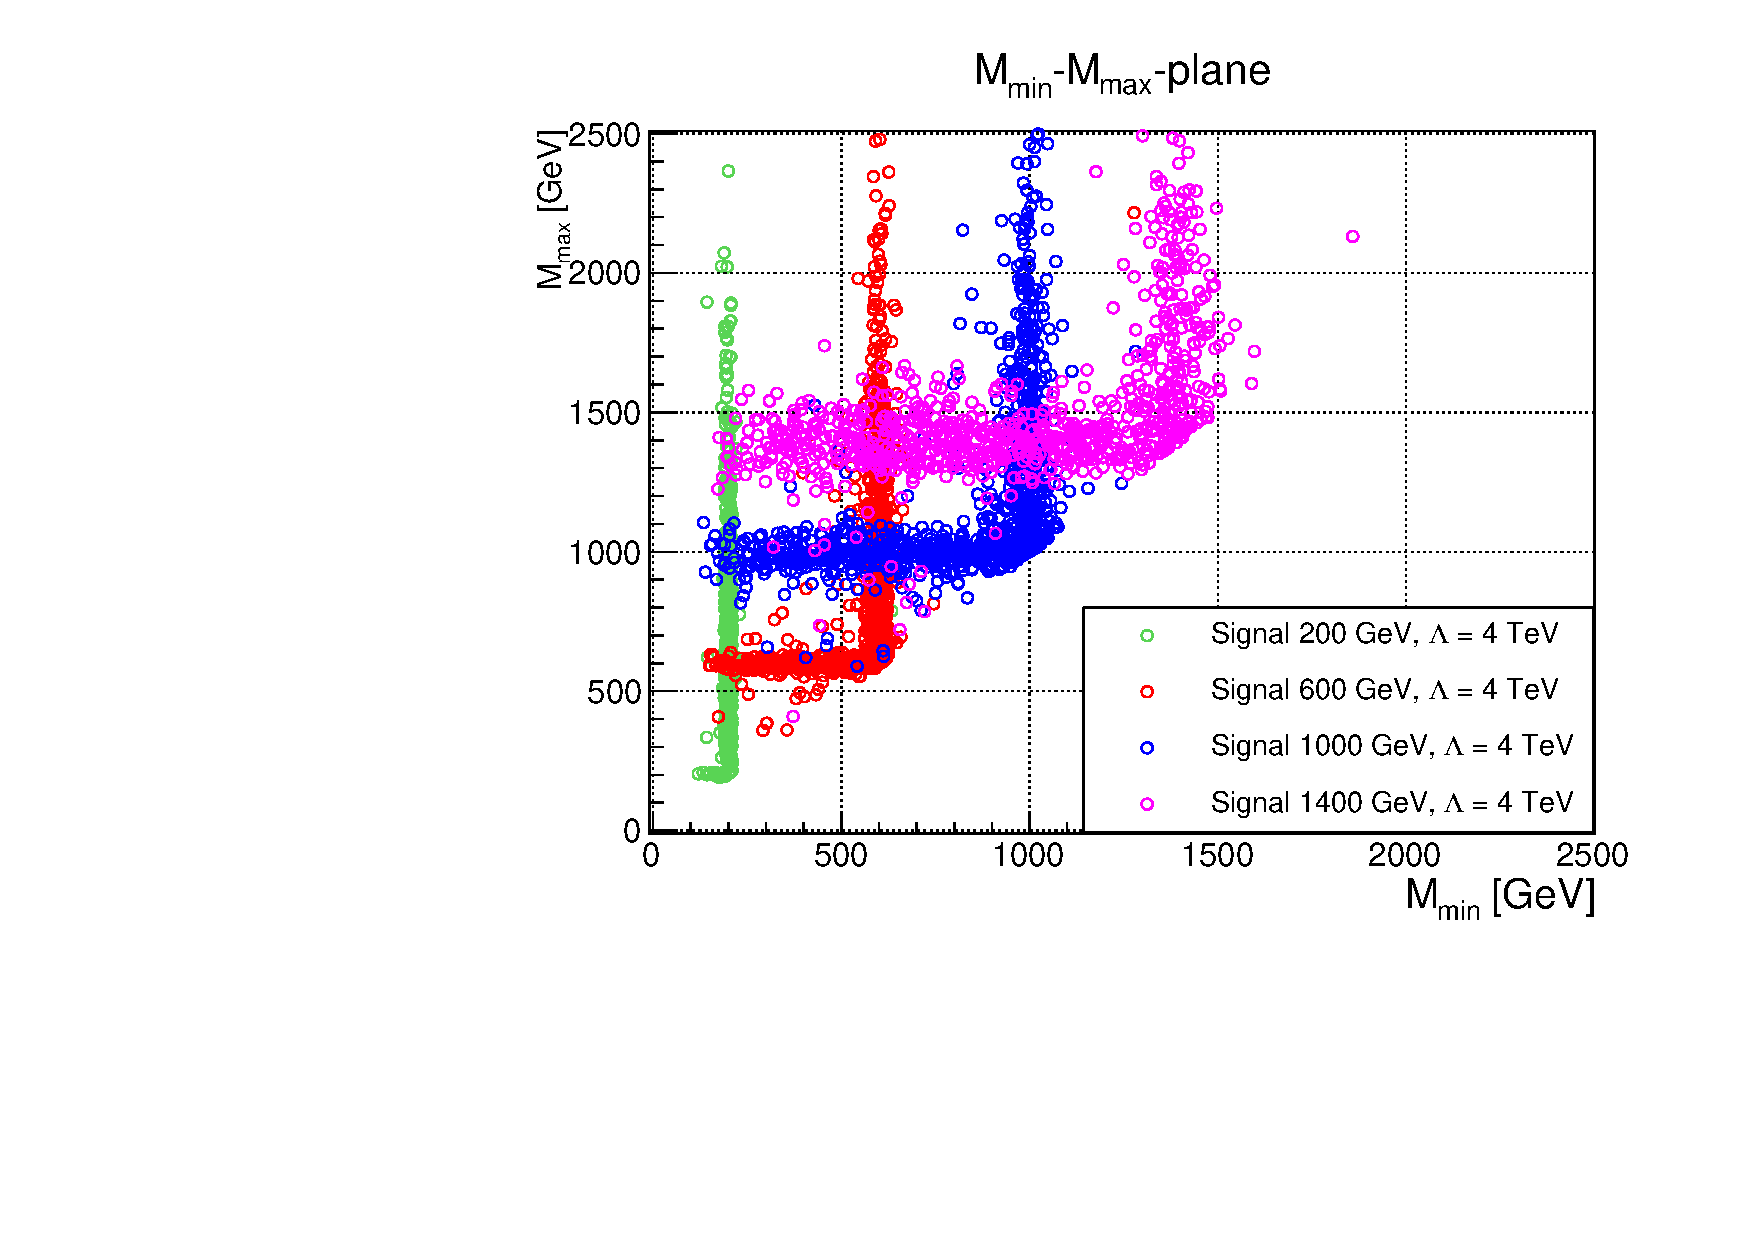
\includegraphics[width=0.48\textwidth]{plot/signal_2mu2e.pdf} 
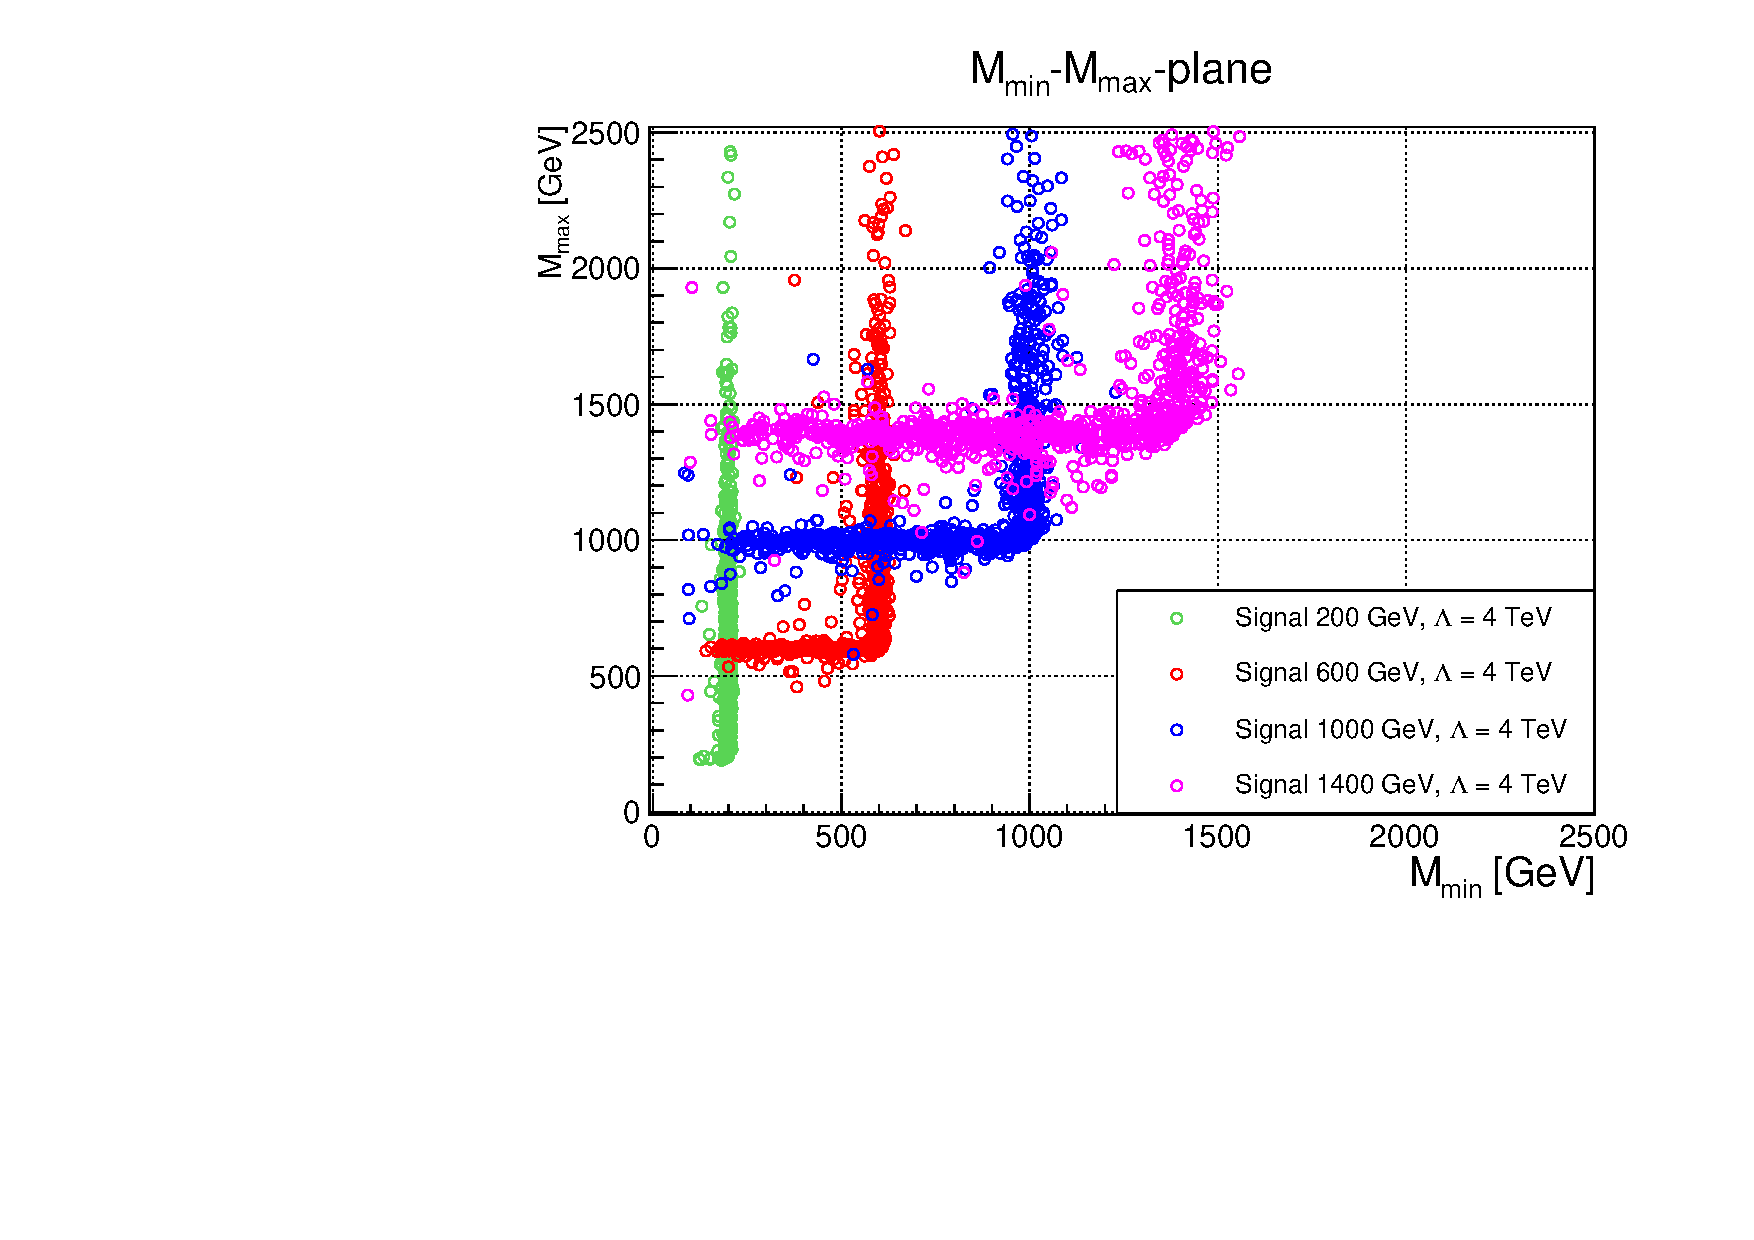
\includegraphics[width=0.48\textwidth]{plot/signal_2e2mu.pdf}
\end{center}
\caption{\label{fig:MminMmaxSignal}2-dimensional minimum-maximum invariant mass distribution after invariant mass cuts for different $l^{*}$ masses. Left: $\mu\mu^{*}\rightarrow 2\mu 2e$ channel. Right: $ee^{*}\rightarrow 2e2\mu$ channel.}
\end{figure}

The boundaries of the final selection depend on the mass of the excited leptons. Fig. \ref{fig:Boundaries} shows the selection of the boundaries for an invariant mass of 600 GeV. There are four cuts set: A lower cut von $M_{min}$, a higher cut on $M_{min}$, a lower cut on $M_{max}$ and a higher cut on $M_{max}$. The most important cuts of this four are the higher $M_{min}$ and the lower $M_{max}$ cuts, which do most effort on seperating signal and background. For the definition of the cut ranges, the best expected limit for the lower maximum invariant mass cut was calculated. Now, a range from optimized lower $M_{max}$ cut to the central mass of each $l^{*}$ samples is obtained. Then, we apply this range to upper $M_{max}$ cut, upper $M_{min}$ cut, and lower $M_{min}$ cut to form a symmetric signal region for each signal sample. Tab. \ref{tab:LShape2} - \ref{tab:LShape4} show the range and the event yields for the different $l^{*}$ masses and Fig. \ref{fig:Efficiencies_L} shows the acceptance $\times$ efficiency after lepton selection, after the Z-veto selection and after the final selection.

\begin{figure}
 \begin{center}
  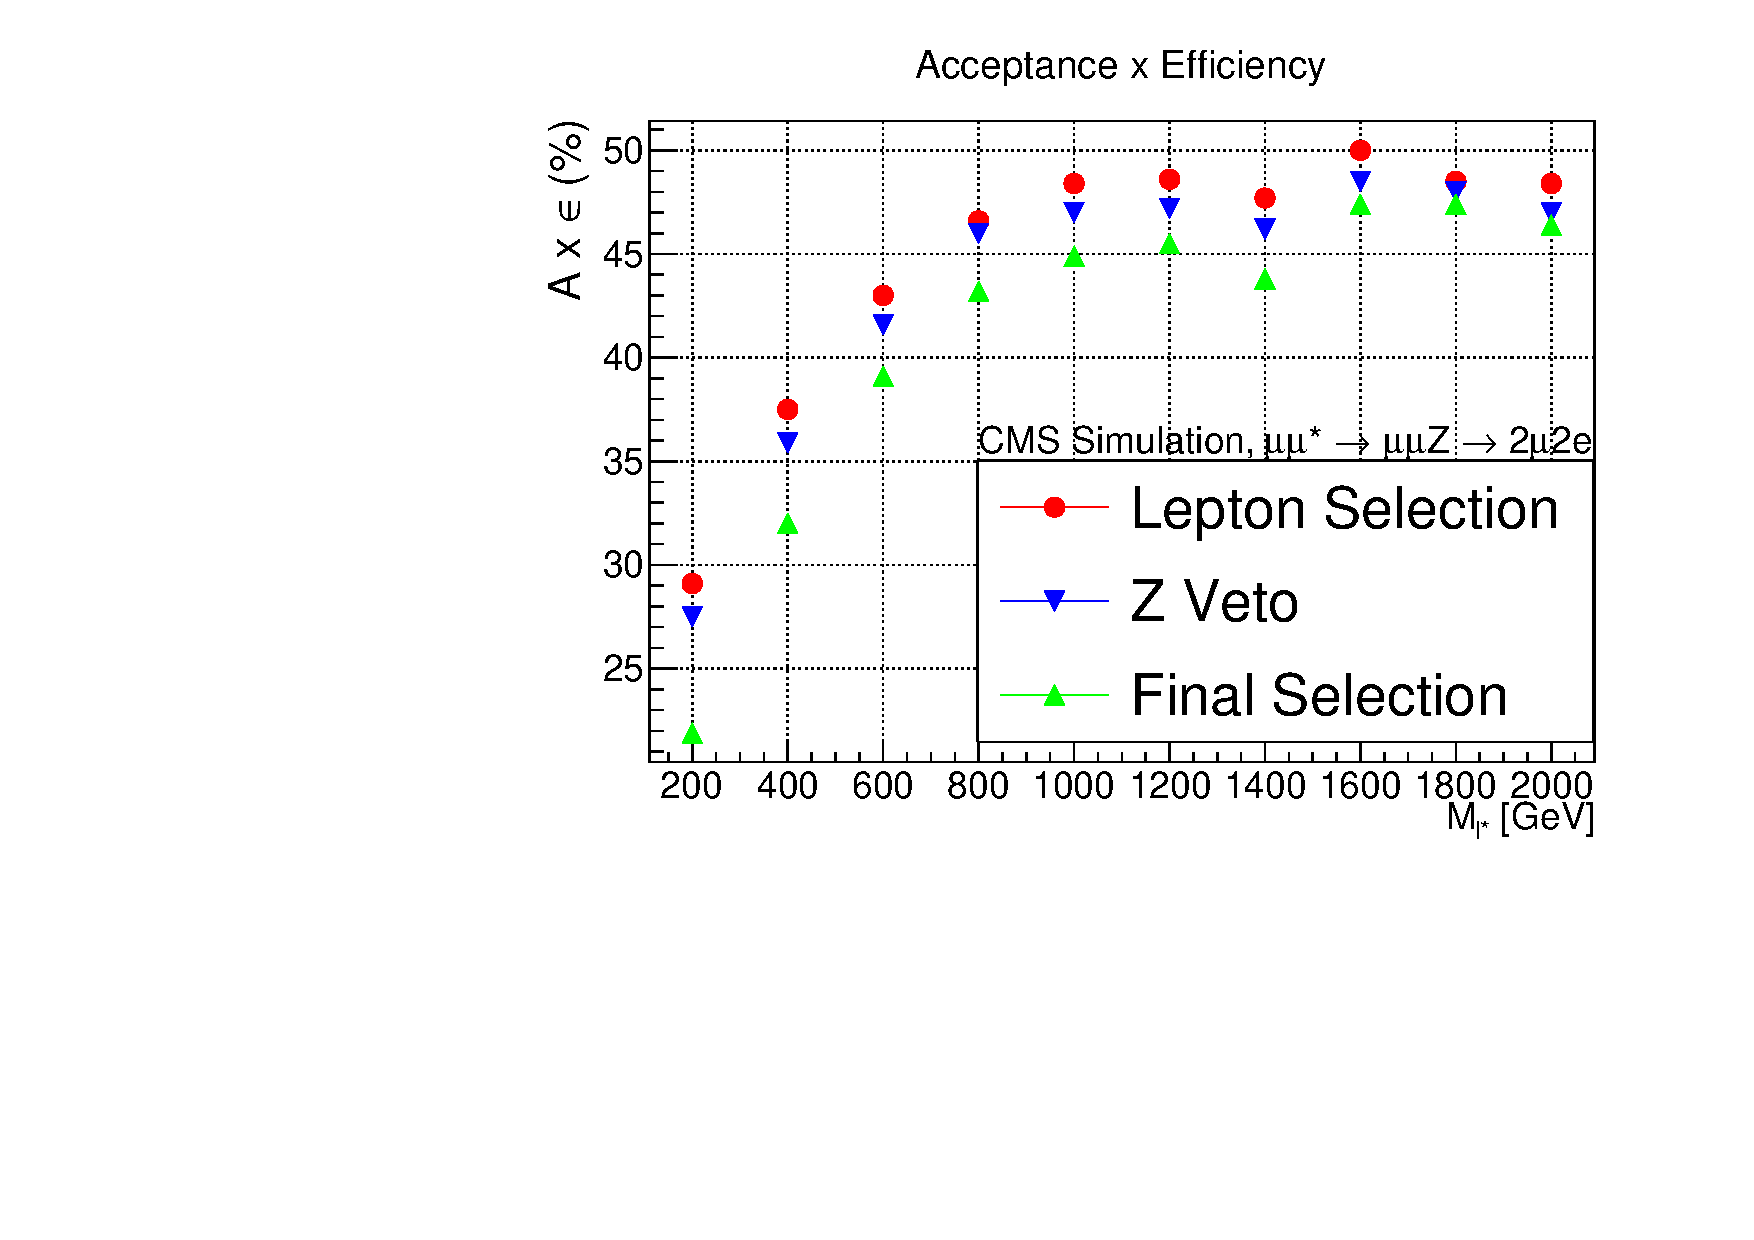
\includegraphics[width=0.48\textwidth]{plot/Effizienz_2mu2e.pdf}
  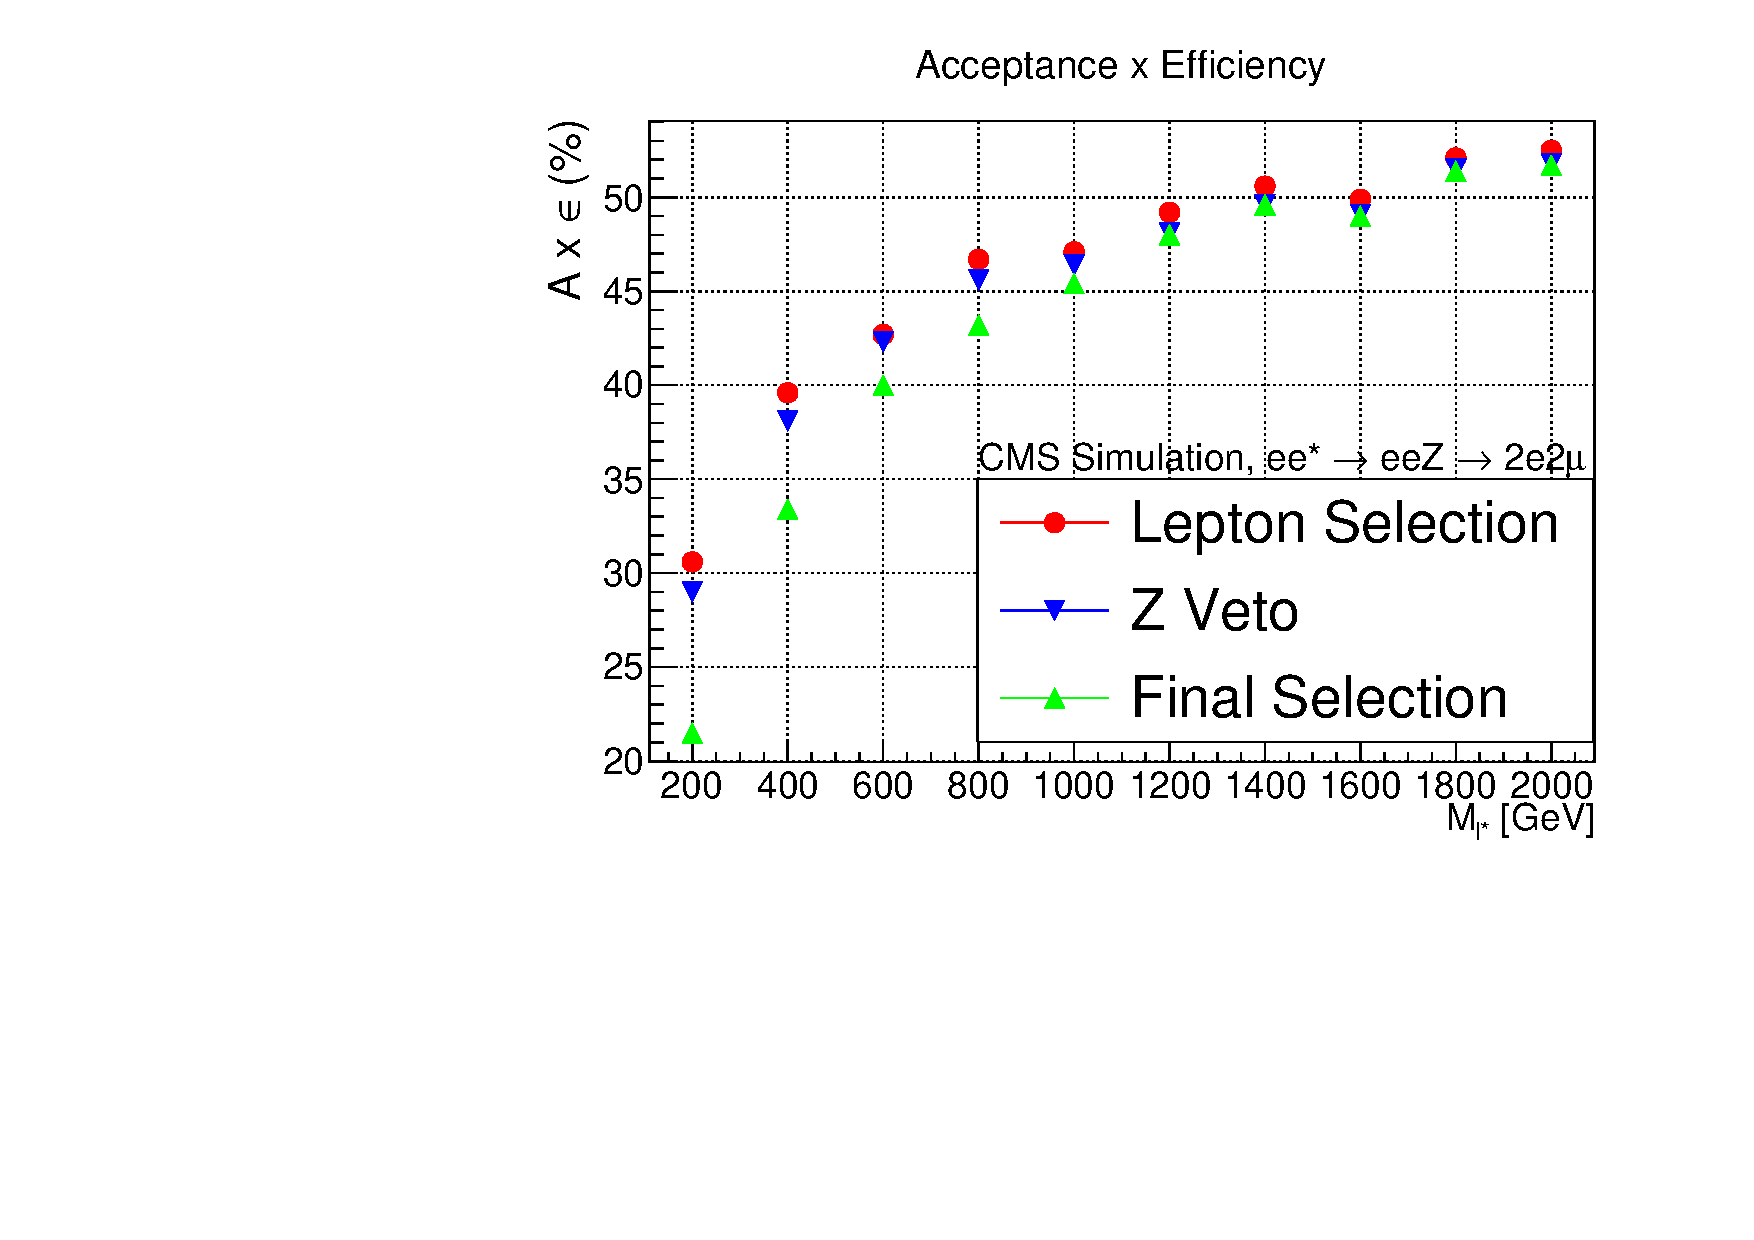
\includegraphics[width=0.48\textwidth]{plot/Effizienz_2e2mu.pdf}
 \end{center}
\caption{\label{fig:Efficiencies_L}Acceptance $\times$ Efficiency for different cut stages: Lepton selection, Z veto and final selection. }
\end{figure}



\begin{table}[h!]
\begin{center}
\begin{tabular}{|l|c|c|c|c|c|}
\hline
m($\mu^{*}$) [GeV] & $M_{min}-M_{max}$ Cut [GeV] & Data & BG (\# Events) & $\epsilon_{all}$ \\
\hline
\hline
200 & 196-204 & 0 & 0.23 $\pm$ 0.05 & 22.3\% \\
400 & 376-424 & 1 & 0.14$\pm$ 0.03 & 32.8\% \\
600 & 540-660 & 0 & 0.07 $\pm$ 0.03 & 39.8\% \\
800 & 720-880 & 0 & 0.04 $\pm$ 0.01 & 44.3\% \\
1000 & 850-1150 & 0 & 0.01 $\pm$ 0.01 & 46.1\% \\
1200 & 1000-1400 & 0 & 0.00 $\pm$ 0.00 & 46.7\% \\
1400 & 1200-1800 & 0 & 0.01 $\pm$ 0.01 & 45.0\% \\
1600 & 1200-2200 & 0 & 0.01 $\pm$ 0.01 & 48.4\% \\
1800 & 1200-2600 & 0 & 0.01 $\pm$ 0.01 & 48.7\% \\
2000 & 1200-3000 & 0 & 0.01 $\pm$ 0.01 & 47.6\% \\
2200 & 1200-3400 & 0 & 0.01 $\pm$ 0.01 & 47.4\% \\
2400 & 1200-3800 & 0 & 0.01 $\pm$ 0.01 & 48.2\% \\
2600 & 1200-4200 & 0 & 0.01 $\pm$ 0.01 & 45.5\% \\
\hline
\end{tabular}
\caption{\label{tab:LShape2}Cut ranges for the L shape cuts, corresponding event yields and signal efficiencies $\mu\mu^{*} \rightarrow 2\mu 2e$.}
\end{center}
\end{table} 

\begin{table}[h!]
\begin{center}
\begin{tabular}{|l|c|c|c|c|c|}
\hline
m($e^{*}$) [GeV] & $M_{min}-M_{max}$ Cut [GeV] & Data & BG (\# Events) & $\epsilon_{all}$ \\
\hline
\hline
200 & 196-204 & 0 & 0.24 $\pm$ 0.05 & 22.4\% \\
400 & 384-416 & 0 & 0.09 $\pm$ 0.02 & 34.6\% \\
600 & 552-648 & 0 & 0.08 $\pm$ 0.02 & 41.6\% \\
800 & 728-872 & 0 & 0.02 $\pm$ 0.01 & 44.7\% \\
1000 & 860-1140 & 0 & 0.02 $\pm$ 0.01 & 47.3\% \\
1200 & 860-1540 & 0 & 0.02 $\pm$ 0.01 & 49.7\% \\
1400 & 860-1940 & 0 & 0.02 $\pm$ 0.01 & 51.1\% \\
1600 & 860-2340 & 0 & 0.02 $\pm$ 0.01 & 51.1\% \\
1800 & 860-2740 & 0 & 0.02 $\pm$ 0.01 & 53.7\% \\
2000 & 860-3140 & 0 & 0.02 $\pm$ 0.01 & 53.8\% \\
2200 & 860-3540 & 0 & 0.02 $\pm$ 0.01 & 52.3\% \\
2400 & 860-3940 & 0 & 0.02 $\pm$ 0.01 & 52.8\% \\
2600 & 860-4340 & 0 & 0.02 $\pm$ 0.01 & 52.6\% \\
\hline
\end{tabular}
\caption{\label{tab:LShape4}Cut ranges for the L shape cuts, corresponding event yields and signal efficiencies $e e^{*} \rightarrow 2e 2\mu$.}
\end{center}
\end{table} 


\begin{figure}[hp]
\begin{center}
\includegraphics[width=0.48\textwidth]{plot/L_shape_2mu2e.pdf} 
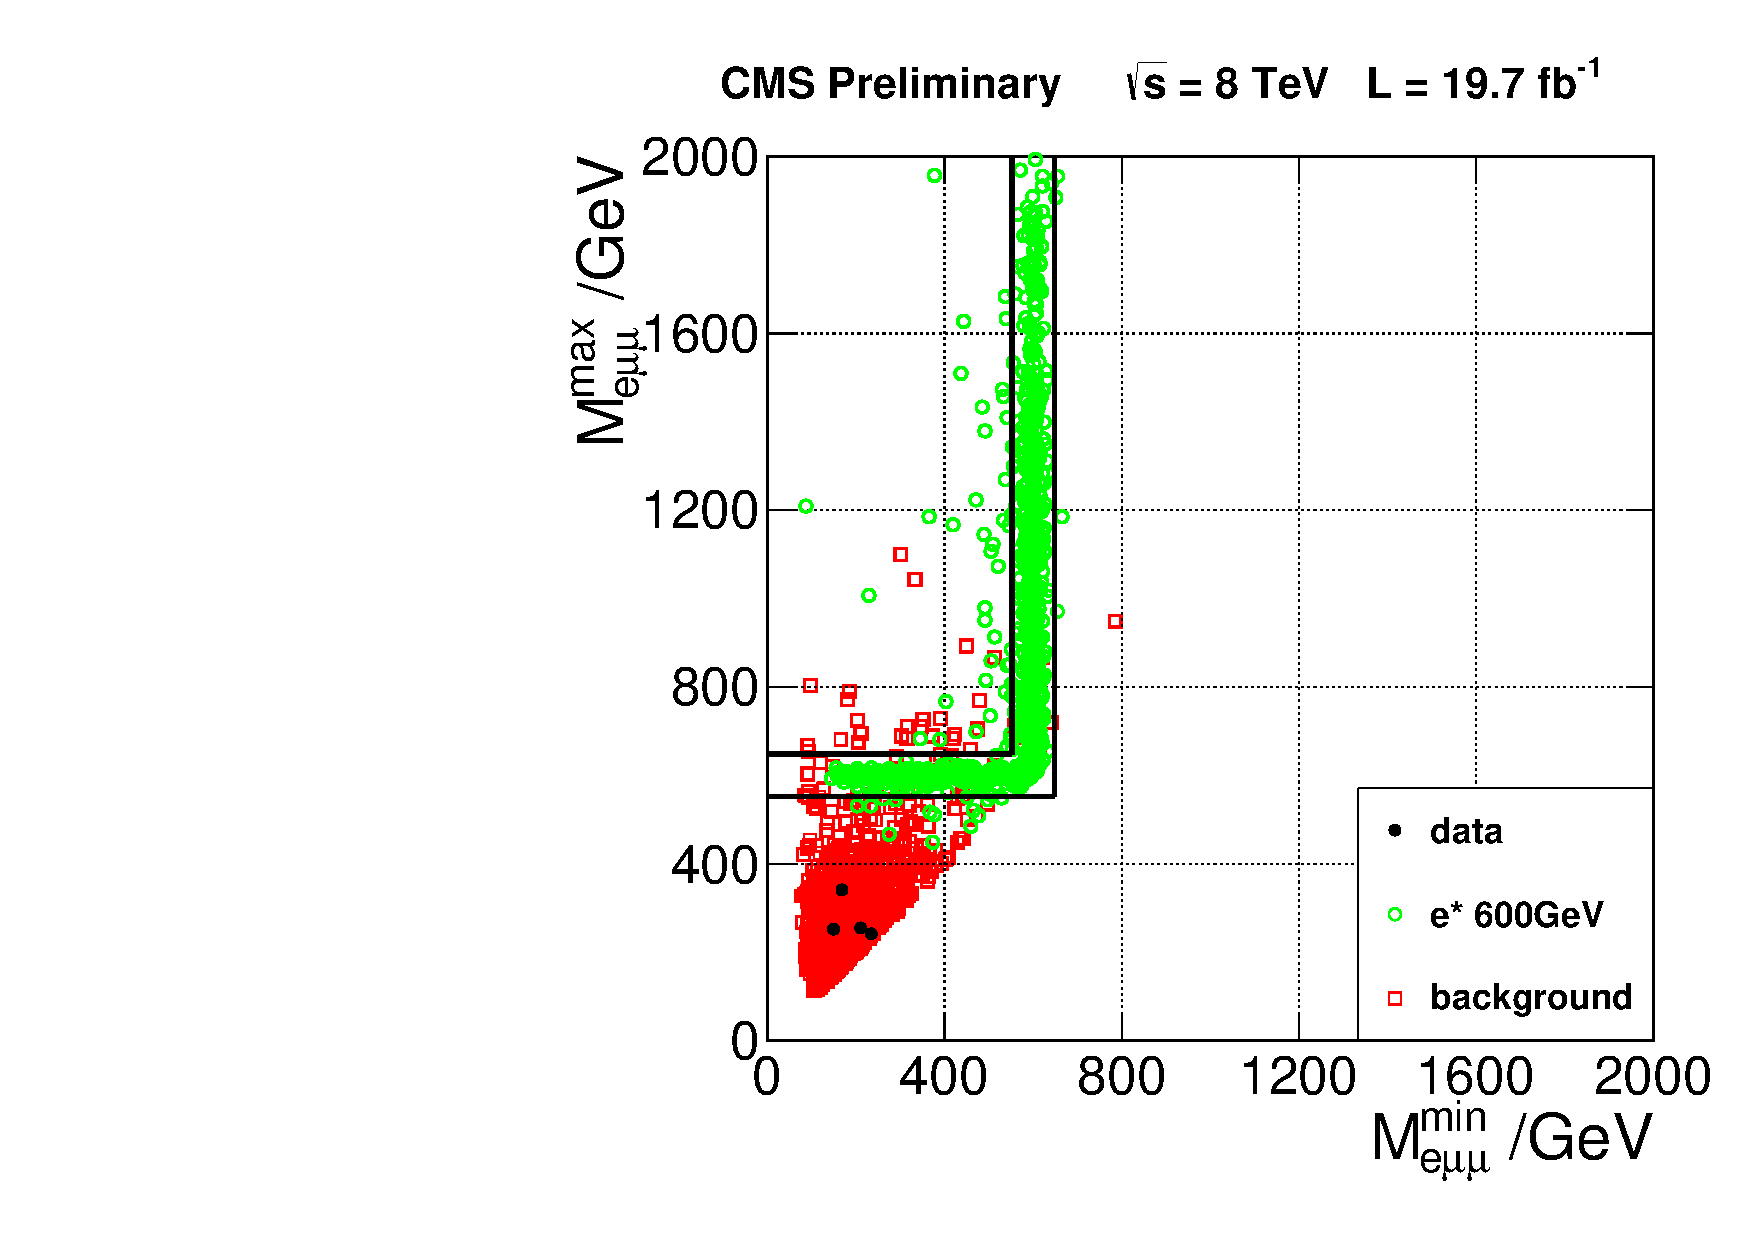
\includegraphics[width=0.48\textwidth]{plot/L_shape_2e2mu.pdf}
\end{center}
\caption{\label{fig:Boundaries}2-dimensional minimum-maximum invariant mass distribution after invariant mass cuts. Left: $\mu\mu^{*} \rightarrow 2\mu 2e$ channel. Right: $ee^{*}\rightarrow 2e2\mu$ channel.}
\end{figure}


Looking at the Tab. \ref{tab:LShape2}-\ref{tab:LShape4}, it can be seen that the selected signal regions do not cover the complete parameter space. Especially in the low mass regions, there are gaps between the search regions that might lead to a case where a potential excited lepton could not be discovered. Those gaps are closed by additional L-shaped search regions that are determined as follows. The 4e-channel is chosen to estimate the new regions as it has the best mass resolution and thus the most narrow windows. For the windows given by the signal MC, the width was plotted depending on the $e^*$-Mass. The width and the position of the new windows is estimated by linear interpolation. The positions are used in all channels, while the correponding width has to be estimated for each channel individually.

Measured data, as well as the background expectation in this new search regions can be drived from the distribution. As there is no corresponding MC, this information is not available for the signal. Estimate the signal contribution by a fit on the points we have from the signal MC. 

The channels containing muons have a much higher A x $\epsilon$ because of the higher efficiency of the high-$p_{T}$ muon ID. As the numbers show, the lose of efficiency due to the L shape cut is very small while we can discriminate the background to a small amount of events. This characteristic returns a very good signal over brackground ratio. 


\section{Limit computation}

The selection defined in section \ref{sec:optimization} and the limit setting tool are used to calculate observed and expected limits for all four channels. The inputs from Tab. \ref{tab:LShape2} - \ref{tab:LShape4} are used for the limit calculation. The calculated cross section limits depend on the compositeness scale $\Lambda$ (here, $f = f^{\prime} = 1$ is assumed). One natural point for limit setting is the point where the $l^{*}$-mass and the compositeness scale have the same value.      

\subsection{Limits for excited muons $\mu^{*}$}

Fig. \ref{fig:limit4mu} and \ref{fig:limit2mu2e} show the cross section limits and the limits on the compositeness scale for $\mu\mu^{*}\rightarrow 4\mu$ and $\mu\mu^{*} 
\rightarrow 2\mu2e$ depending on the $\mu^{*}$-mass. The black lines show the signal cross section for different values of $\Lambda$. From those plots, the channel 
$\mu\mu^{*}\rightarrow 4\mu$ excited muons can be excluded up to a mass of 1.65 TeV for $\Lambda = M_{\mu^{*}}$. In the channel  $\mu\mu^{*}\rightarrow 2\mu2e$, the limit is set to 1.60 TeV. 

\begin{figure}[hp!]
\begin{center}
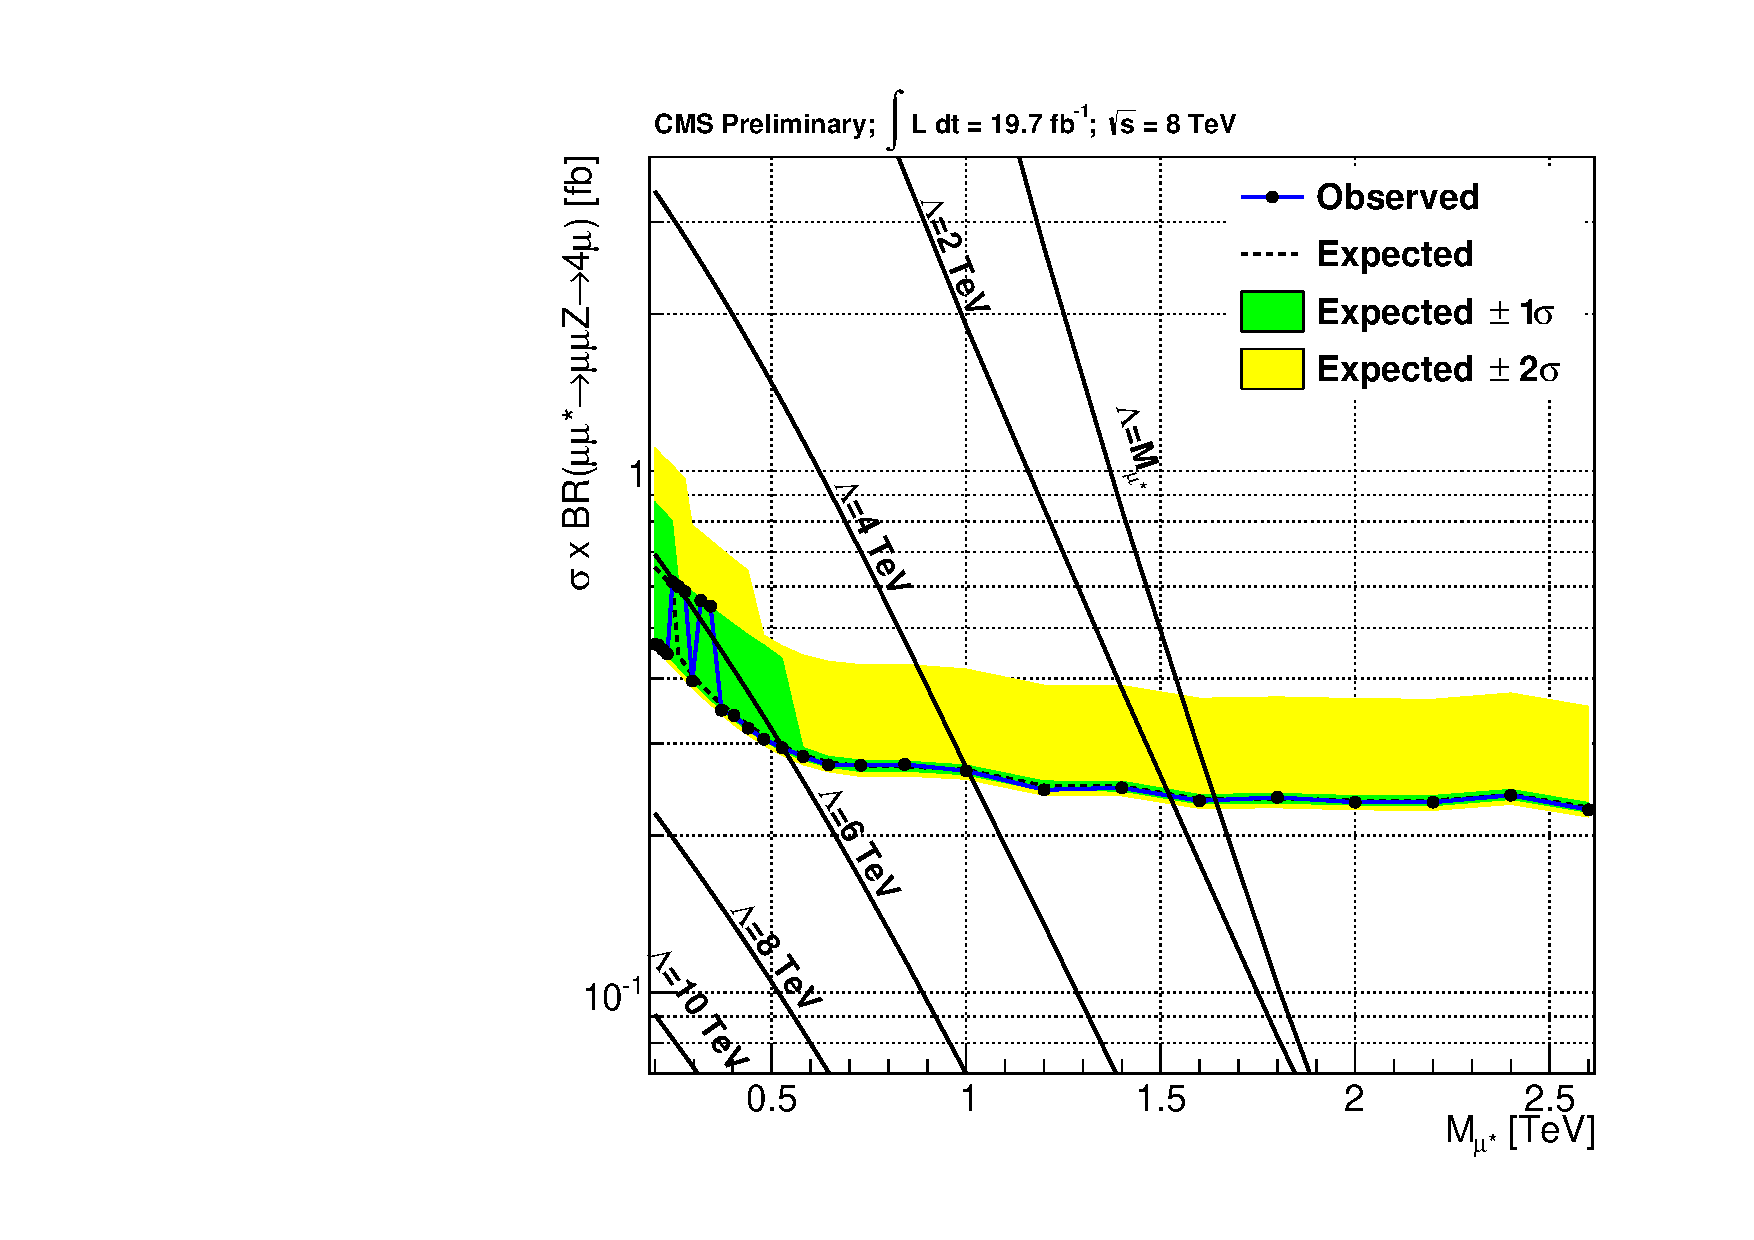
\includegraphics[width=0.48\textwidth]{plot/limit_4mu.pdf}
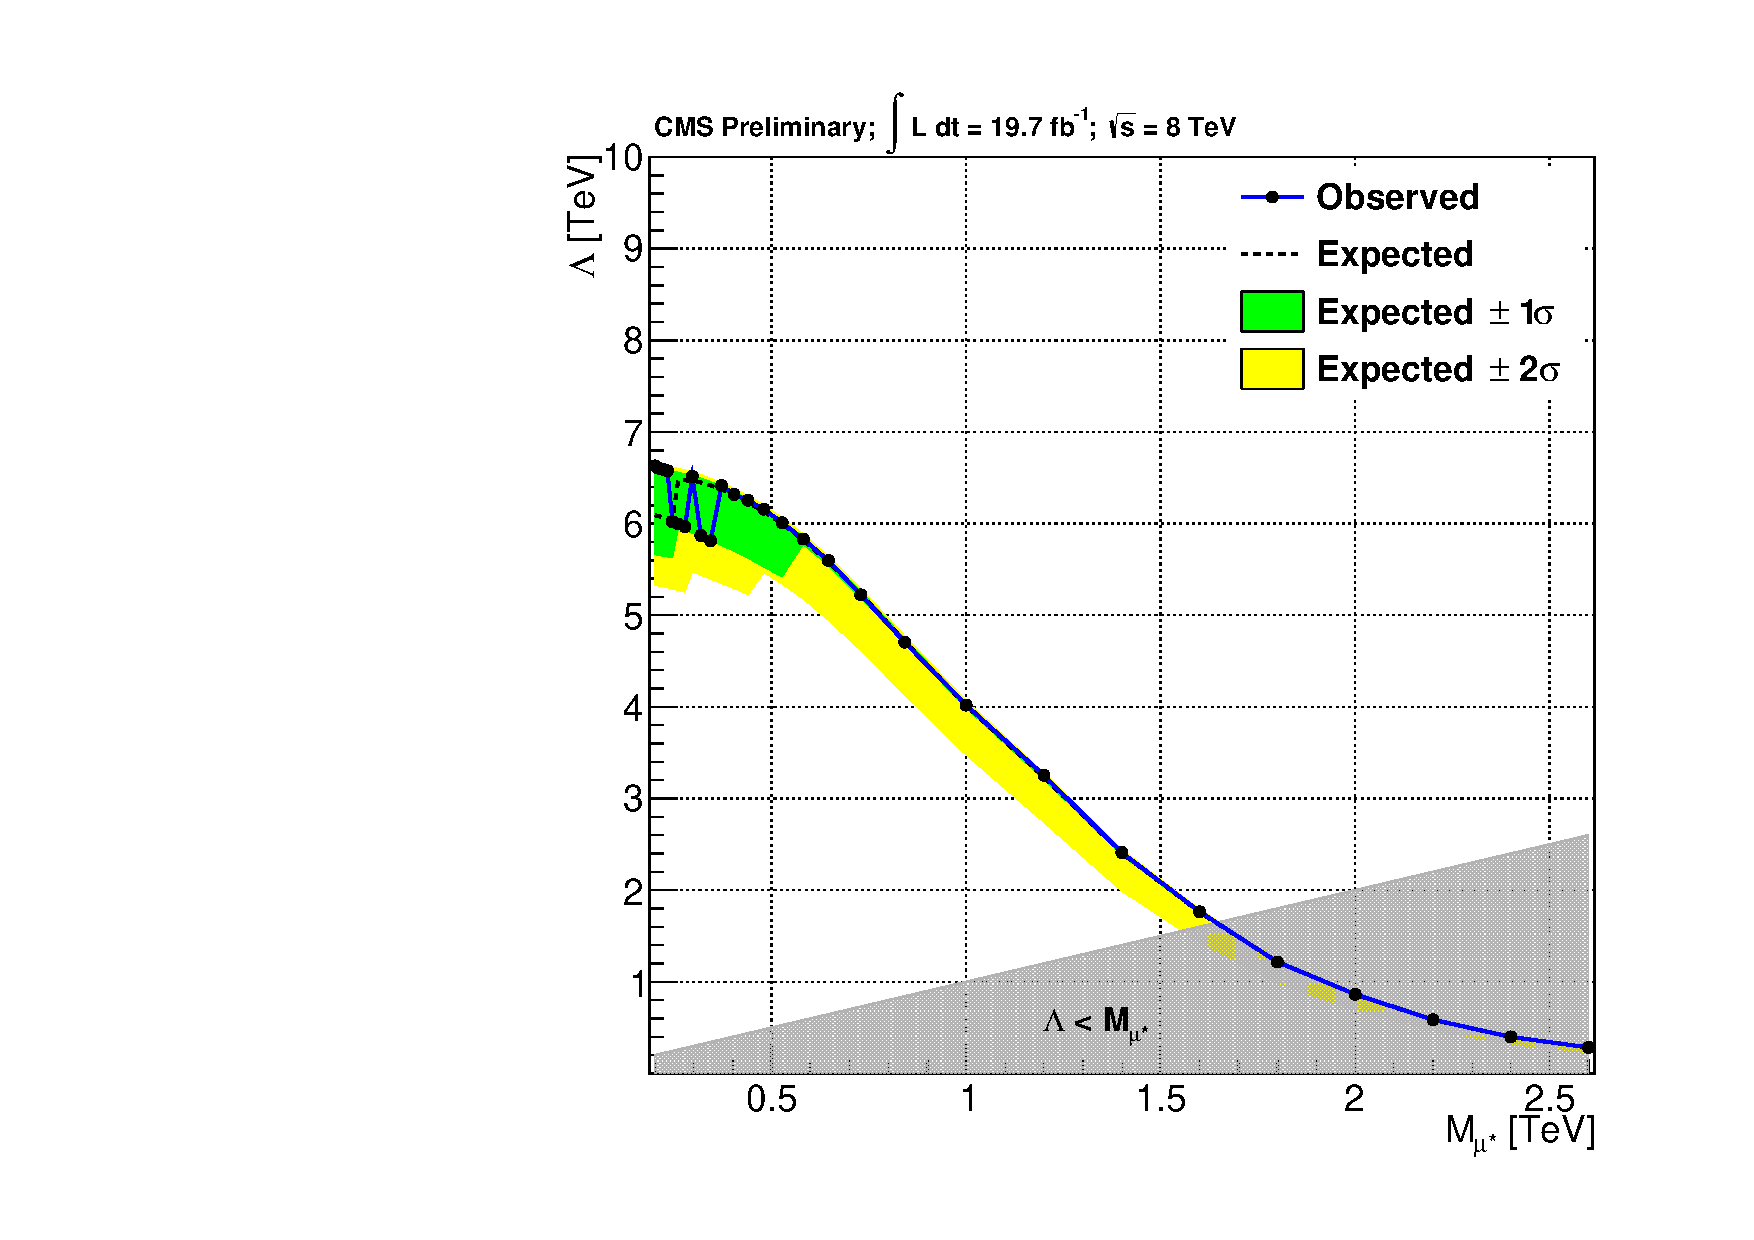
\includegraphics[width=0.48\textwidth]{plot/limit_lambda_4mu.pdf}
\end{center}
\caption{\label{fig:limit4mu}Cross section and $\Lambda$ limit for $\mu\mu^{*} \rightarrow 4\mu$.}
\end{figure}

\begin{figure}[hp!]
\begin{center}
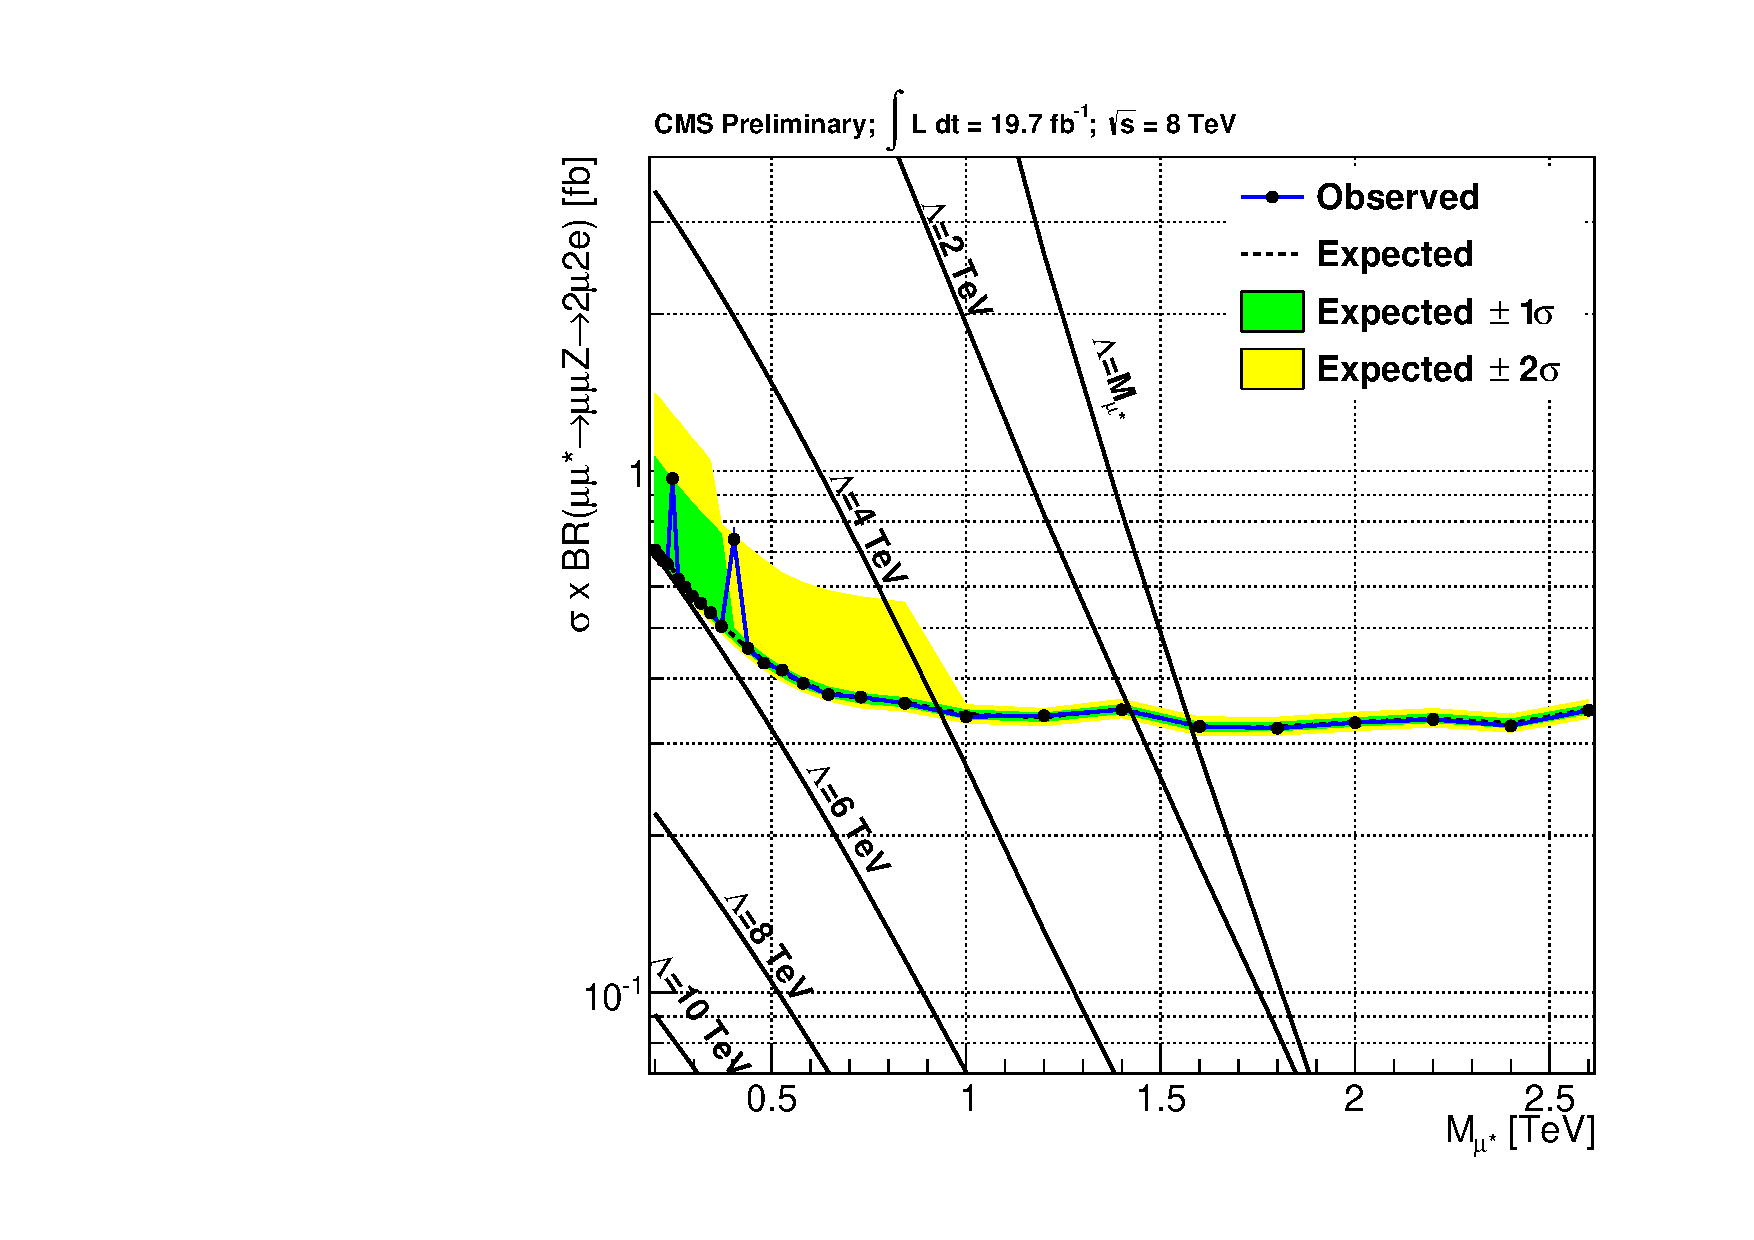
\includegraphics[width=0.48\textwidth]{plot/limit_2mu2e.pdf}
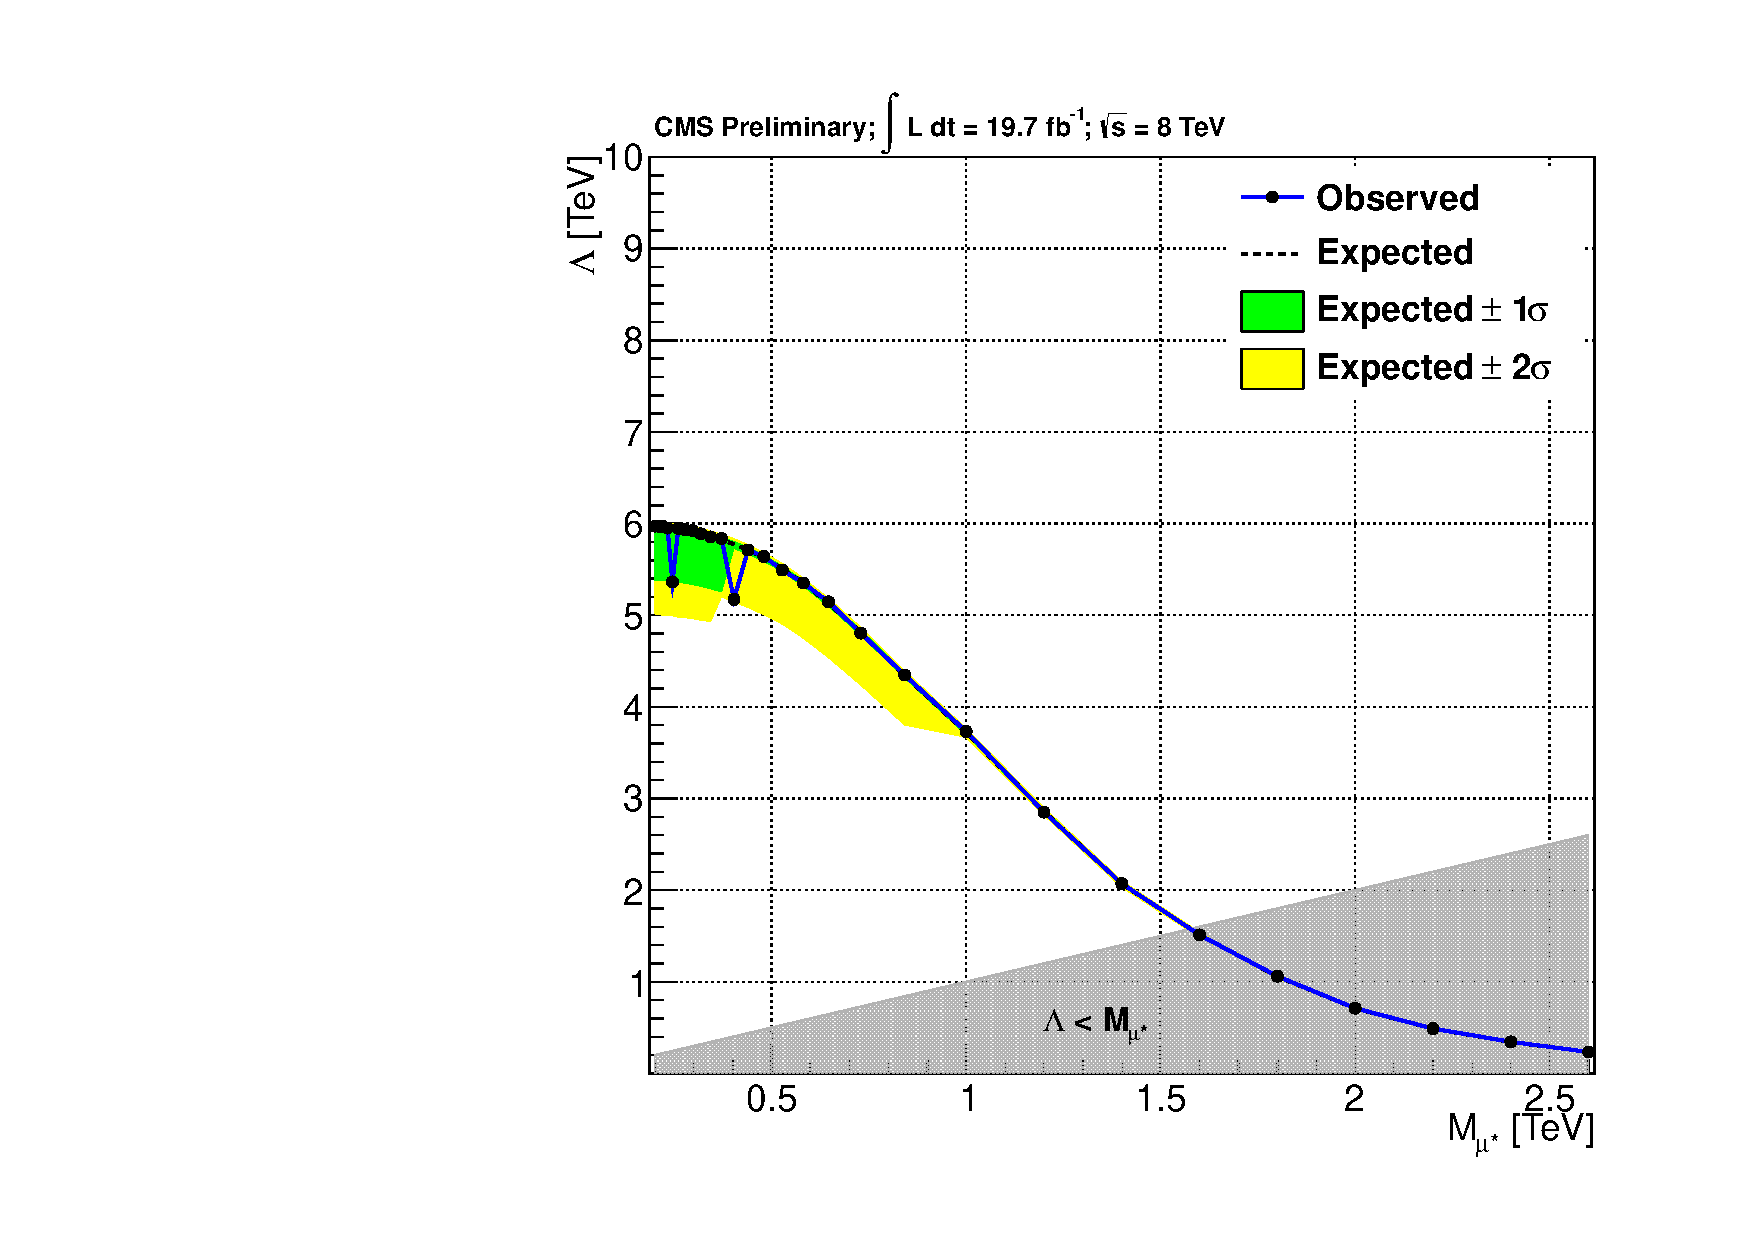
\includegraphics[width=0.48\textwidth]{plot/limit_lambda_2mu2e.pdf}
\end{center}
\caption{\label{fig:limit2mu2e}Cross section and $\Lambda$ limit for $\mu\mu^{*} \rightarrow 2\mu2e$.}
\end{figure}

\subsection{Limits for excited leptons $e^{*}$}

For excited electrons, the same limits as for the excited muons search has been calculated. Fig. \ref{fig:limit4e} and \ref{fig:limit2e2mu} show the cross section limits and the limits on the compositeness scale for $e^{*}\rightarrow 4e$ and $ee^{*} \rightarrow 2e2\mu$. Here, both channels exclud masses up to 1.60 TeV for $\Lambda = M_{e^{*}}$. 

\begin{figure}[hp!]
\begin{center}
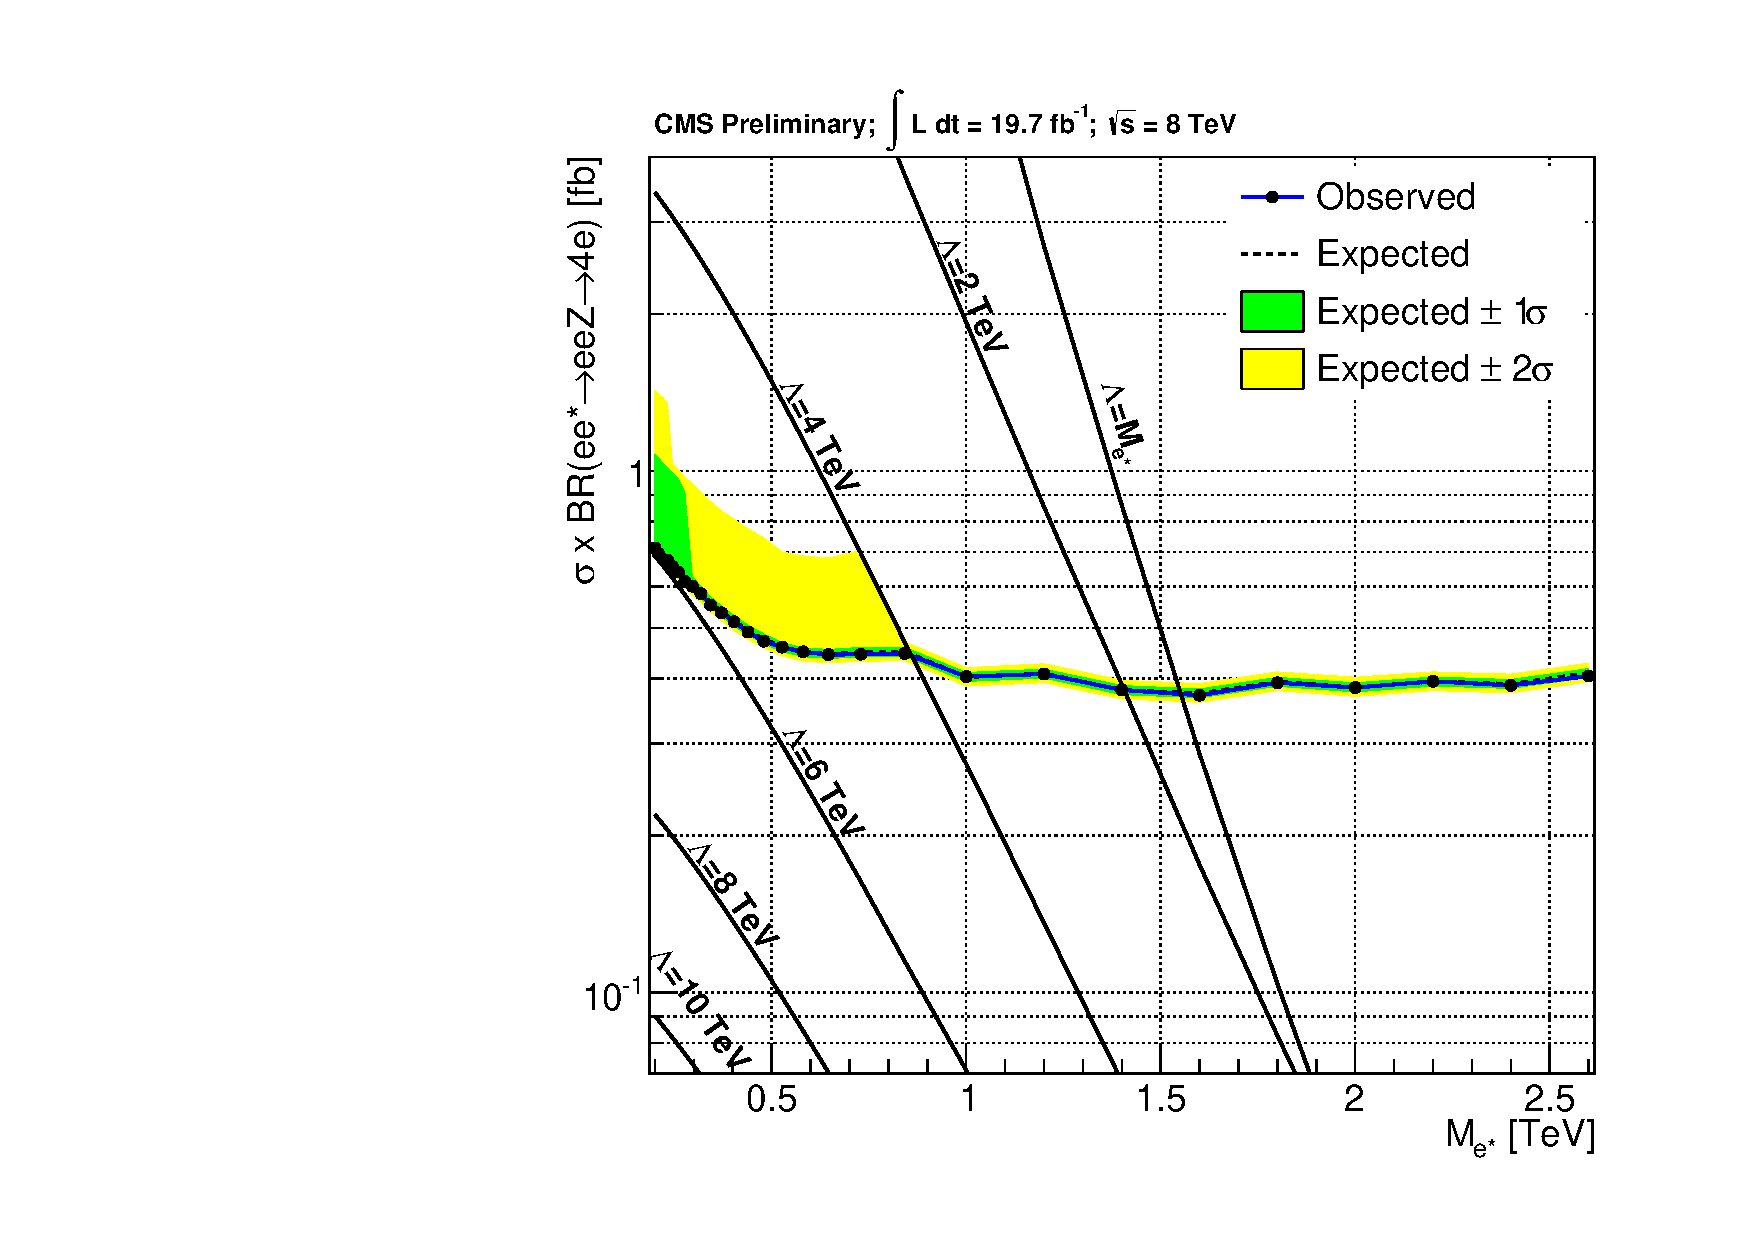
\includegraphics[width=0.48\textwidth]{plot/limit_4e.pdf}
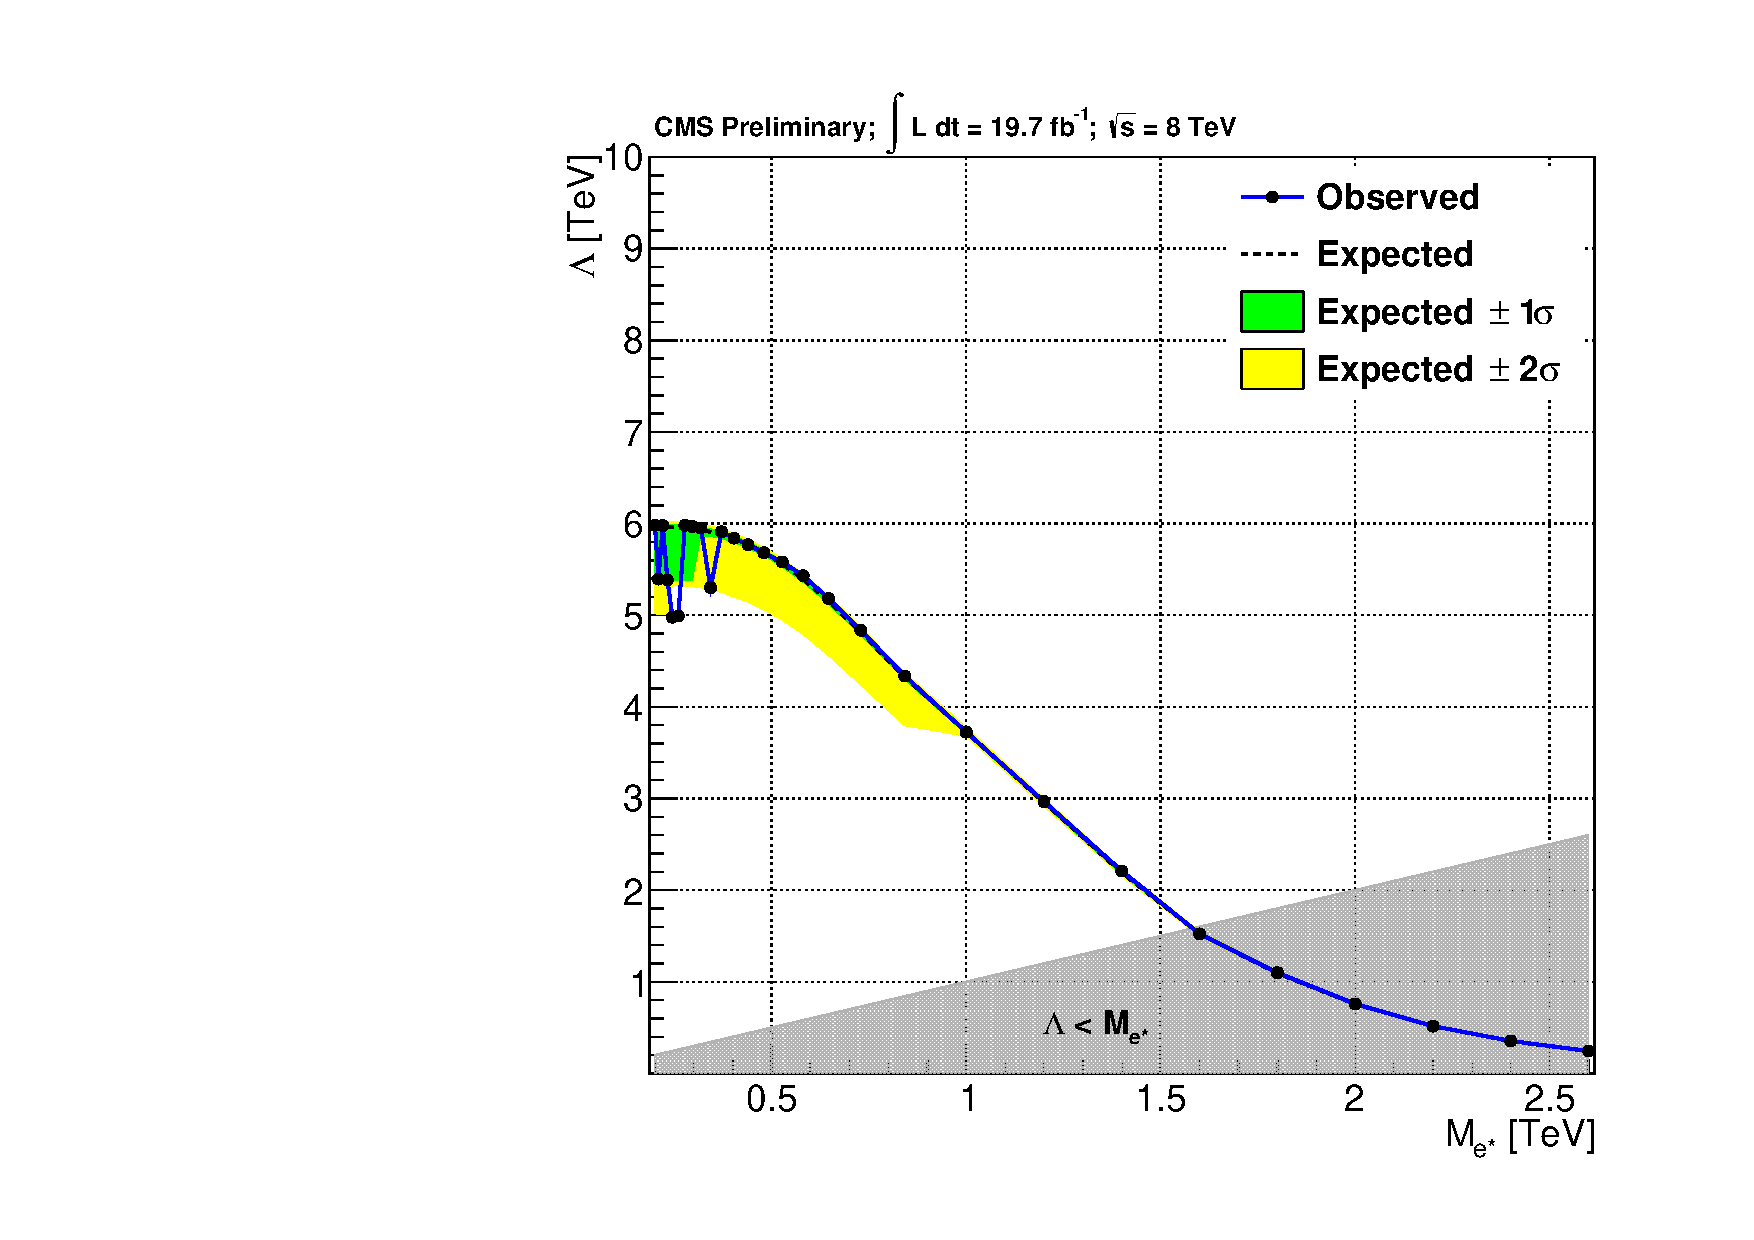
\includegraphics[width=0.48\textwidth]{plot/limit_lambda_2e2mu.pdf}
\end{center}
\caption{\label{fig:limit4e}Cross section and $\Lambda$ limit for $e e^{*} \rightarrow 4e$.}
\end{figure}

\begin{figure}[hp!]
\begin{center}
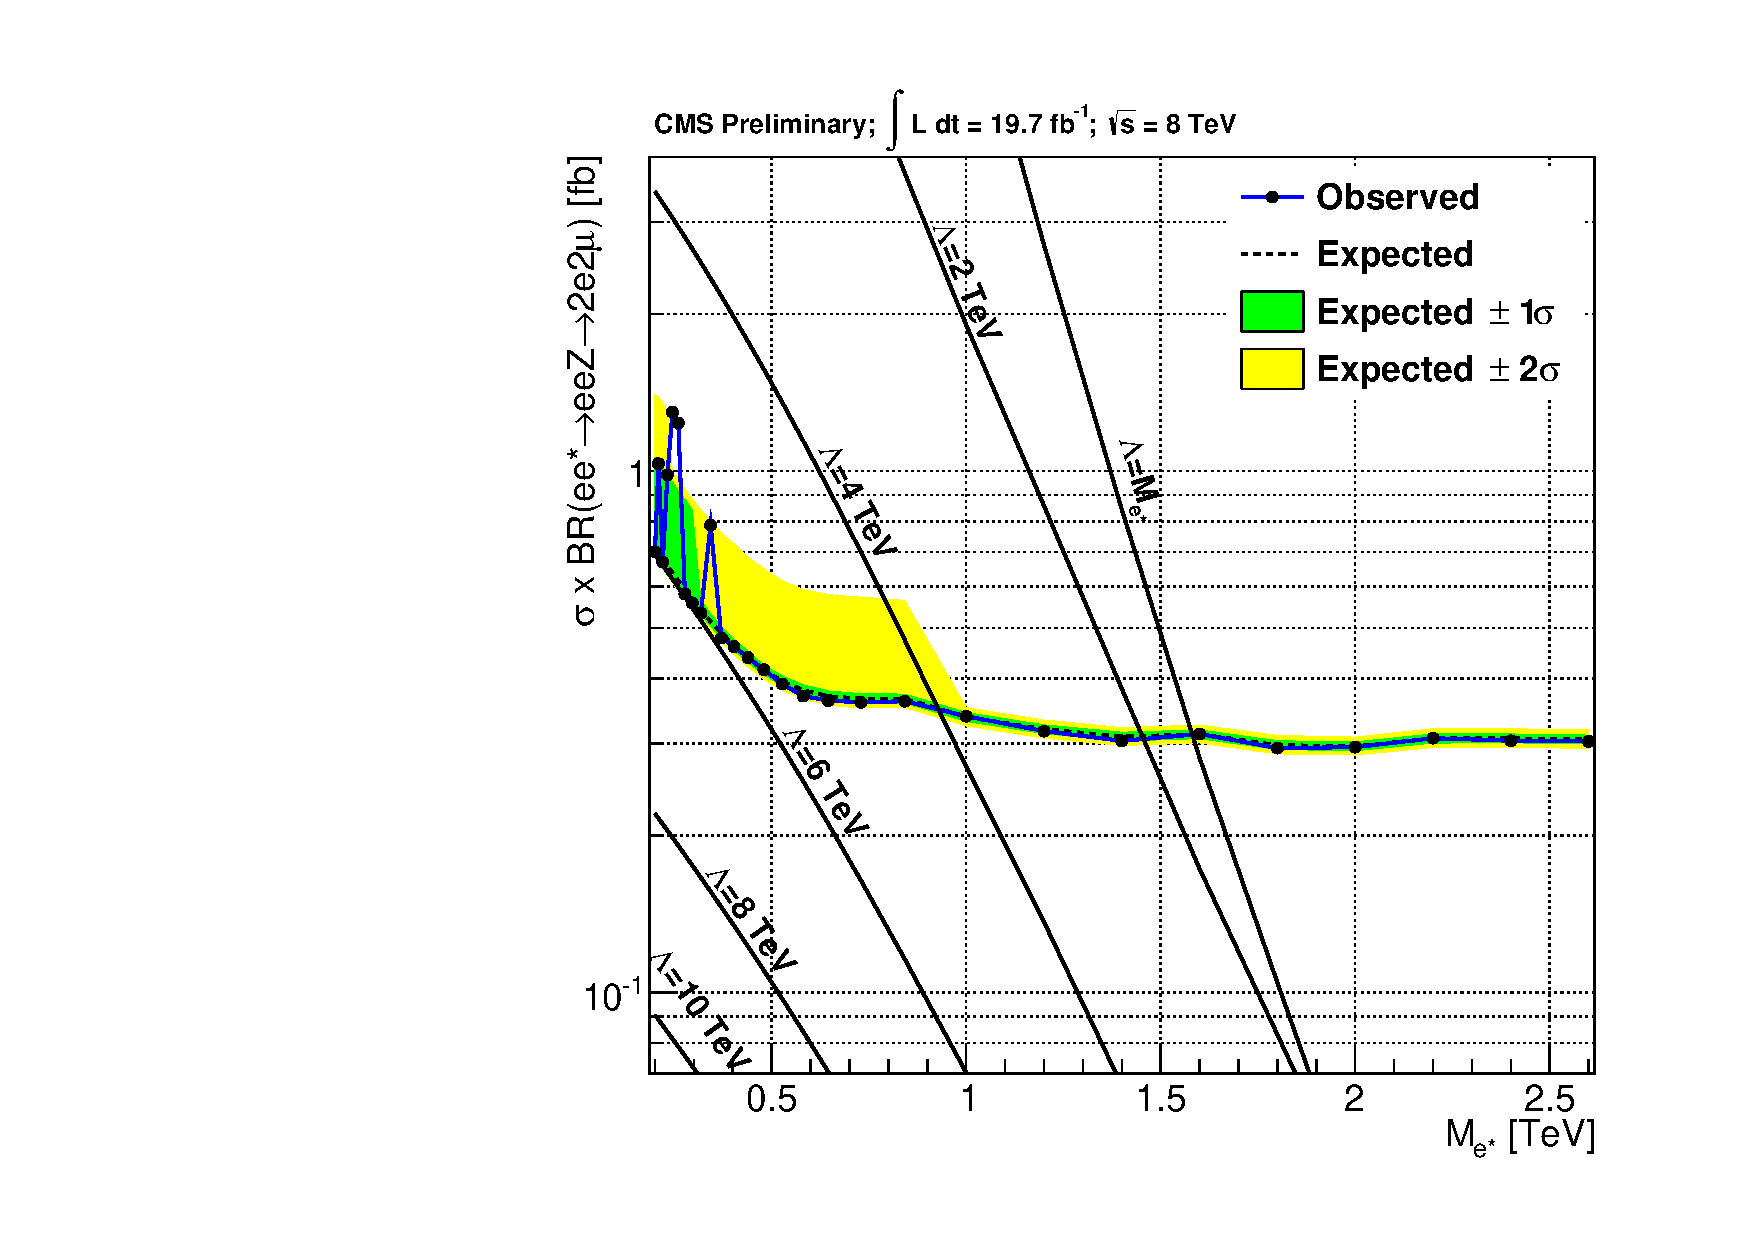
\includegraphics[width=0.48\textwidth]{plot/limit_2e2mu.pdf}
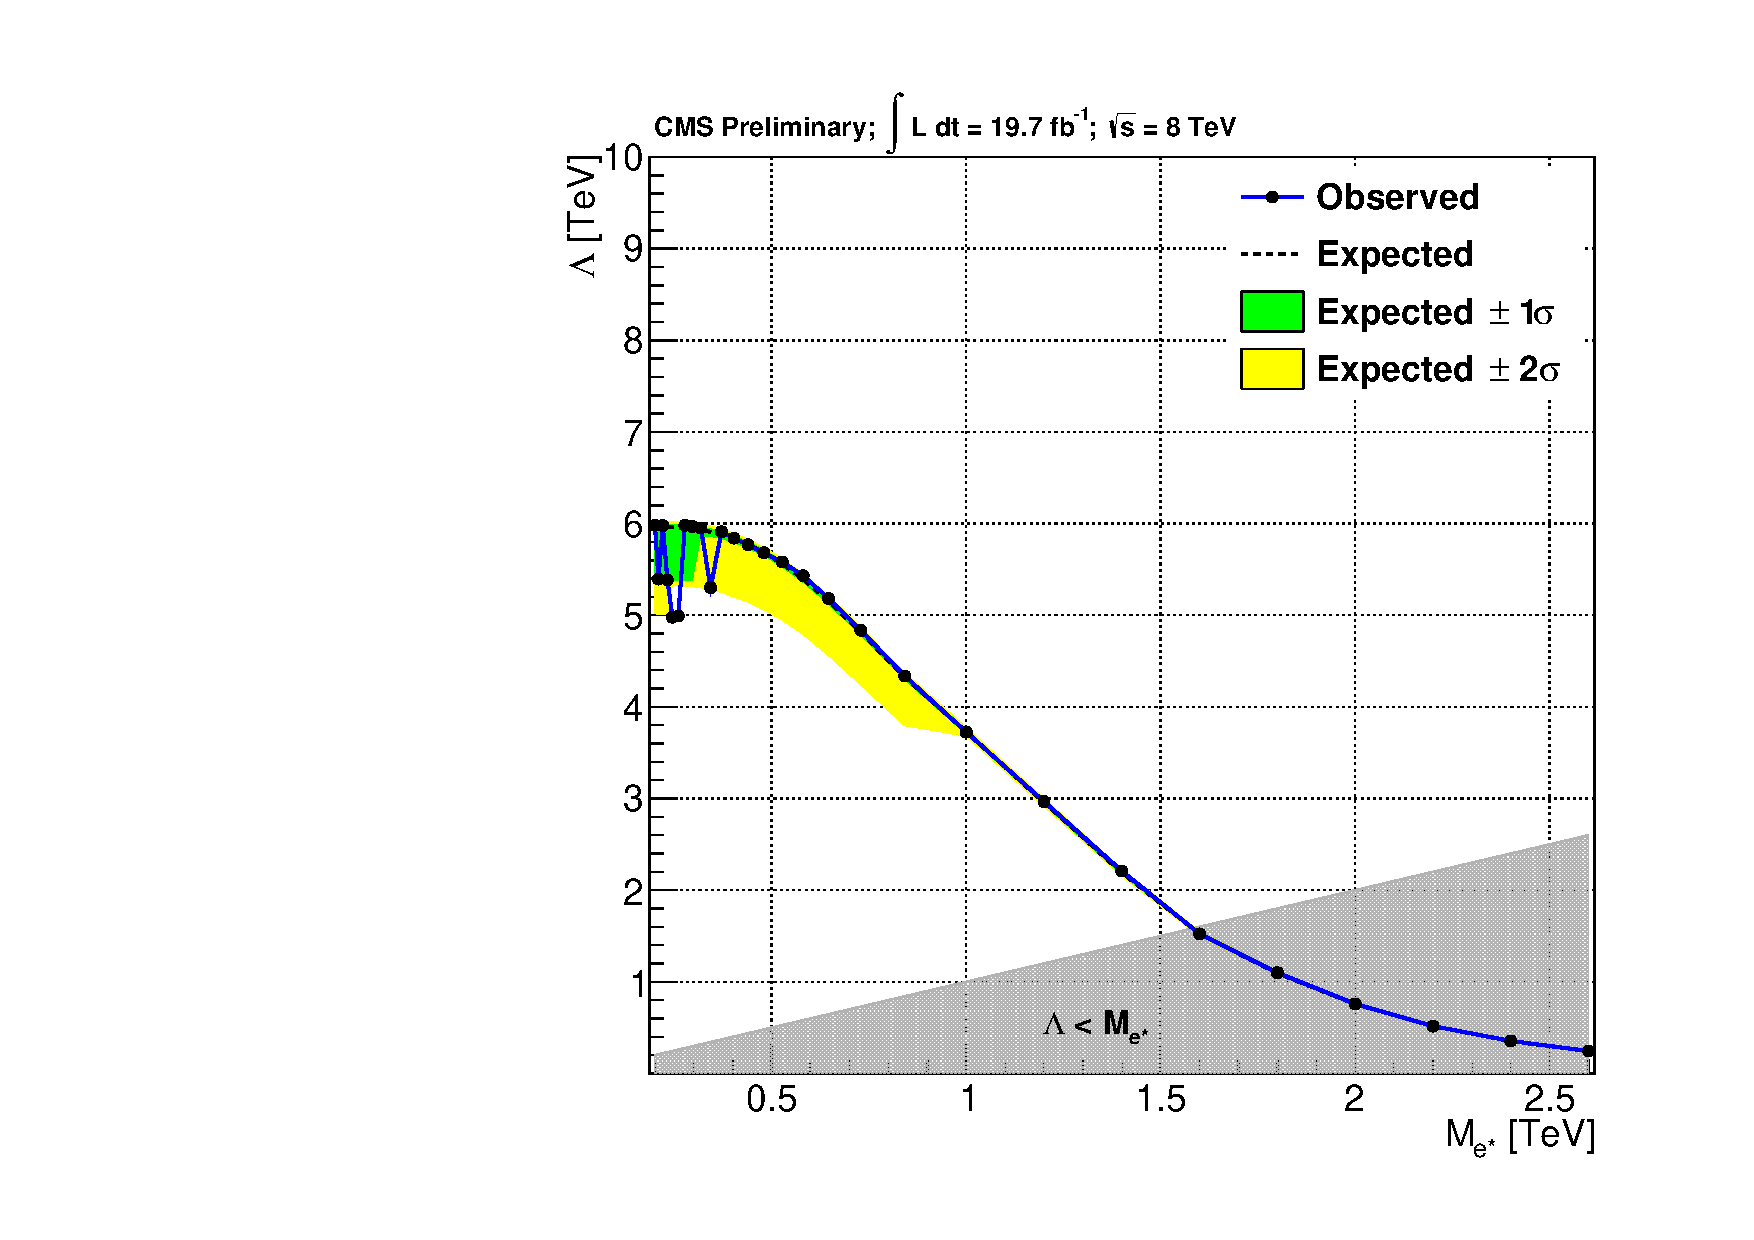
\includegraphics[width=0.48\textwidth]{plot/limit_lambda_2e2mu.pdf}
\end{center}
\caption{\label{fig:limit2e2mu}Cross section and $\Lambda$ limit for $e e^{*} \rightarrow 2e 2\mu$.}
\end{figure}

Depending on the limits of both channels, a combination has been done. This combination leads to an exclusion limit of 1.75 TeV for excited muons from Fig. \ref{fig:limitmustar}. The limit on excited electrons can be set to 1.7 TeV for $\Lambda = M_{e^{*}}$ as shown in \ref{fig:limitestar}. In all cases, the expected and observed limits are close to each other.

\begin{figure}[hp!]
\begin{center}
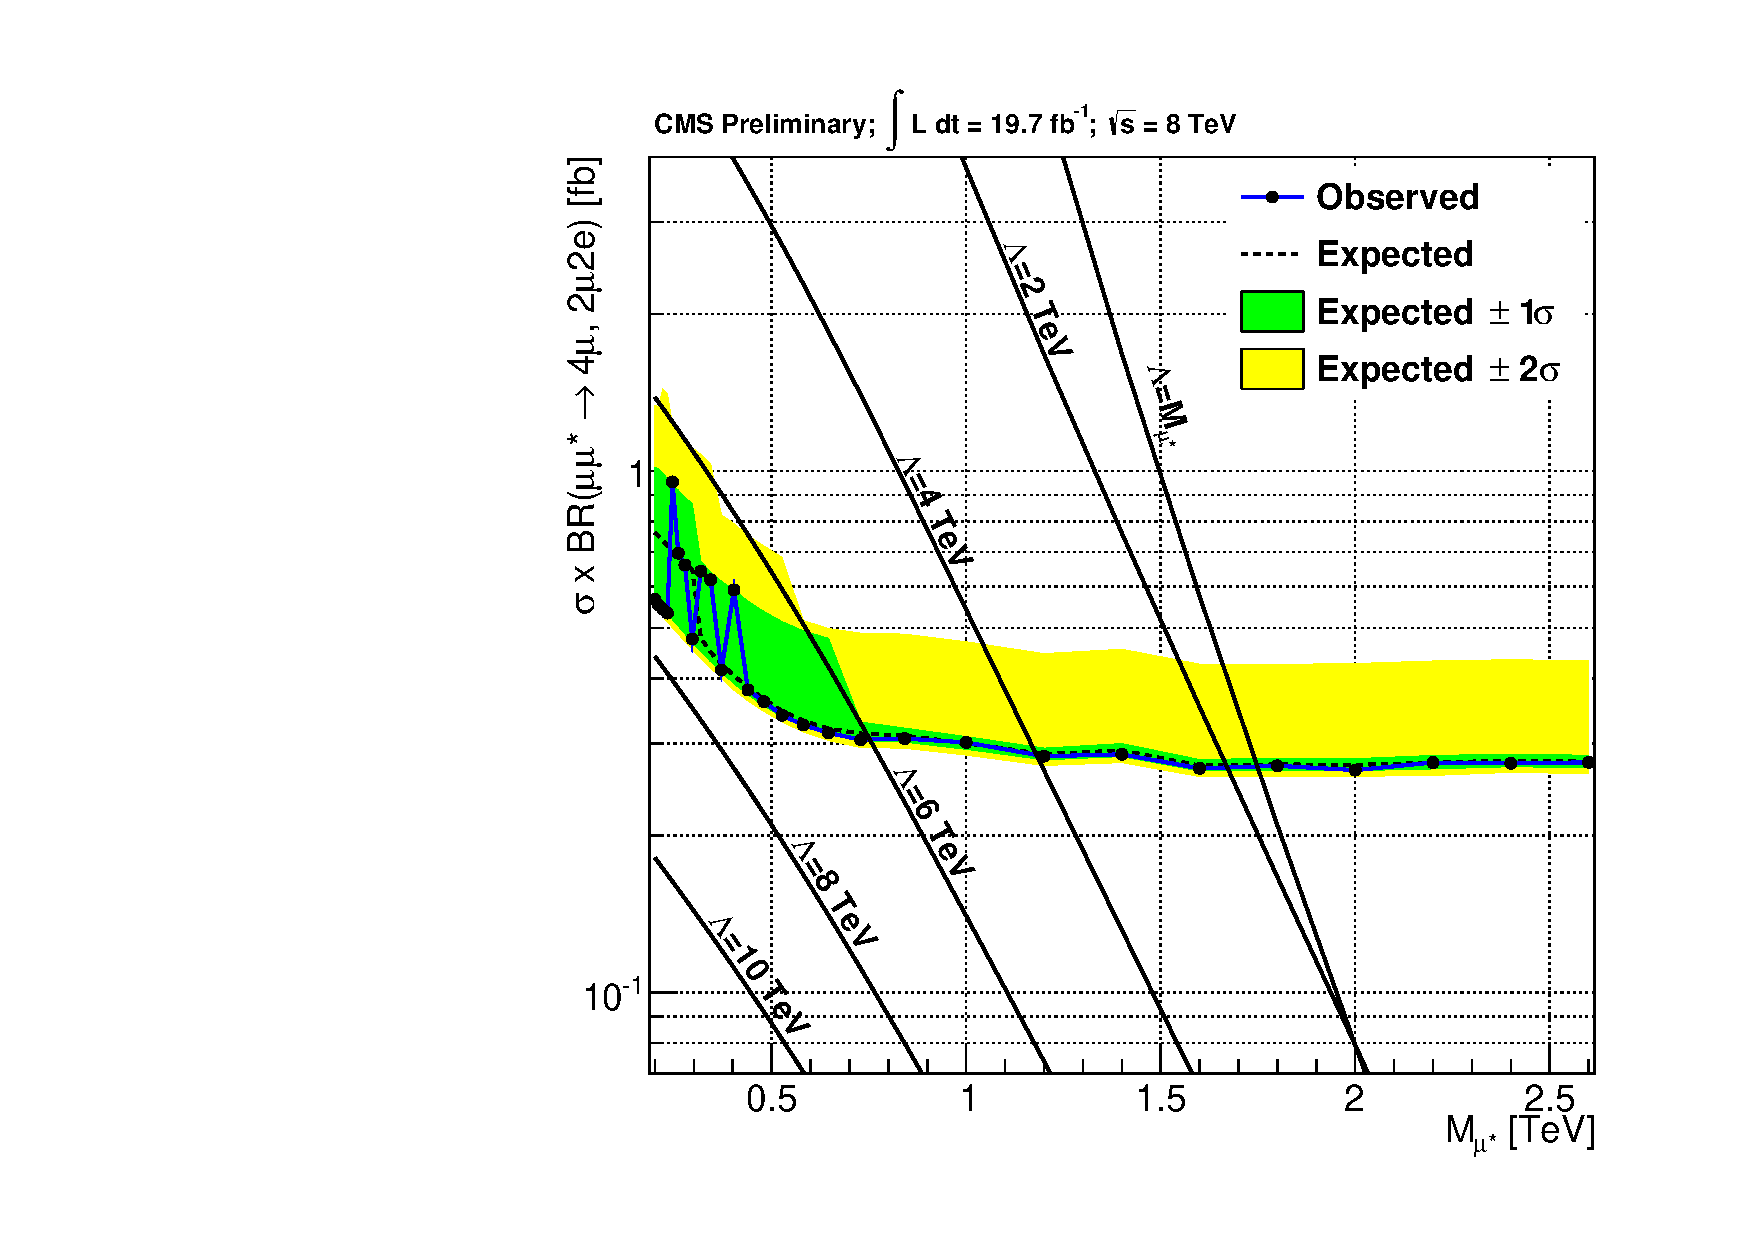
\includegraphics[width=0.48\textwidth]{plot/limit_combined_mustar.pdf}
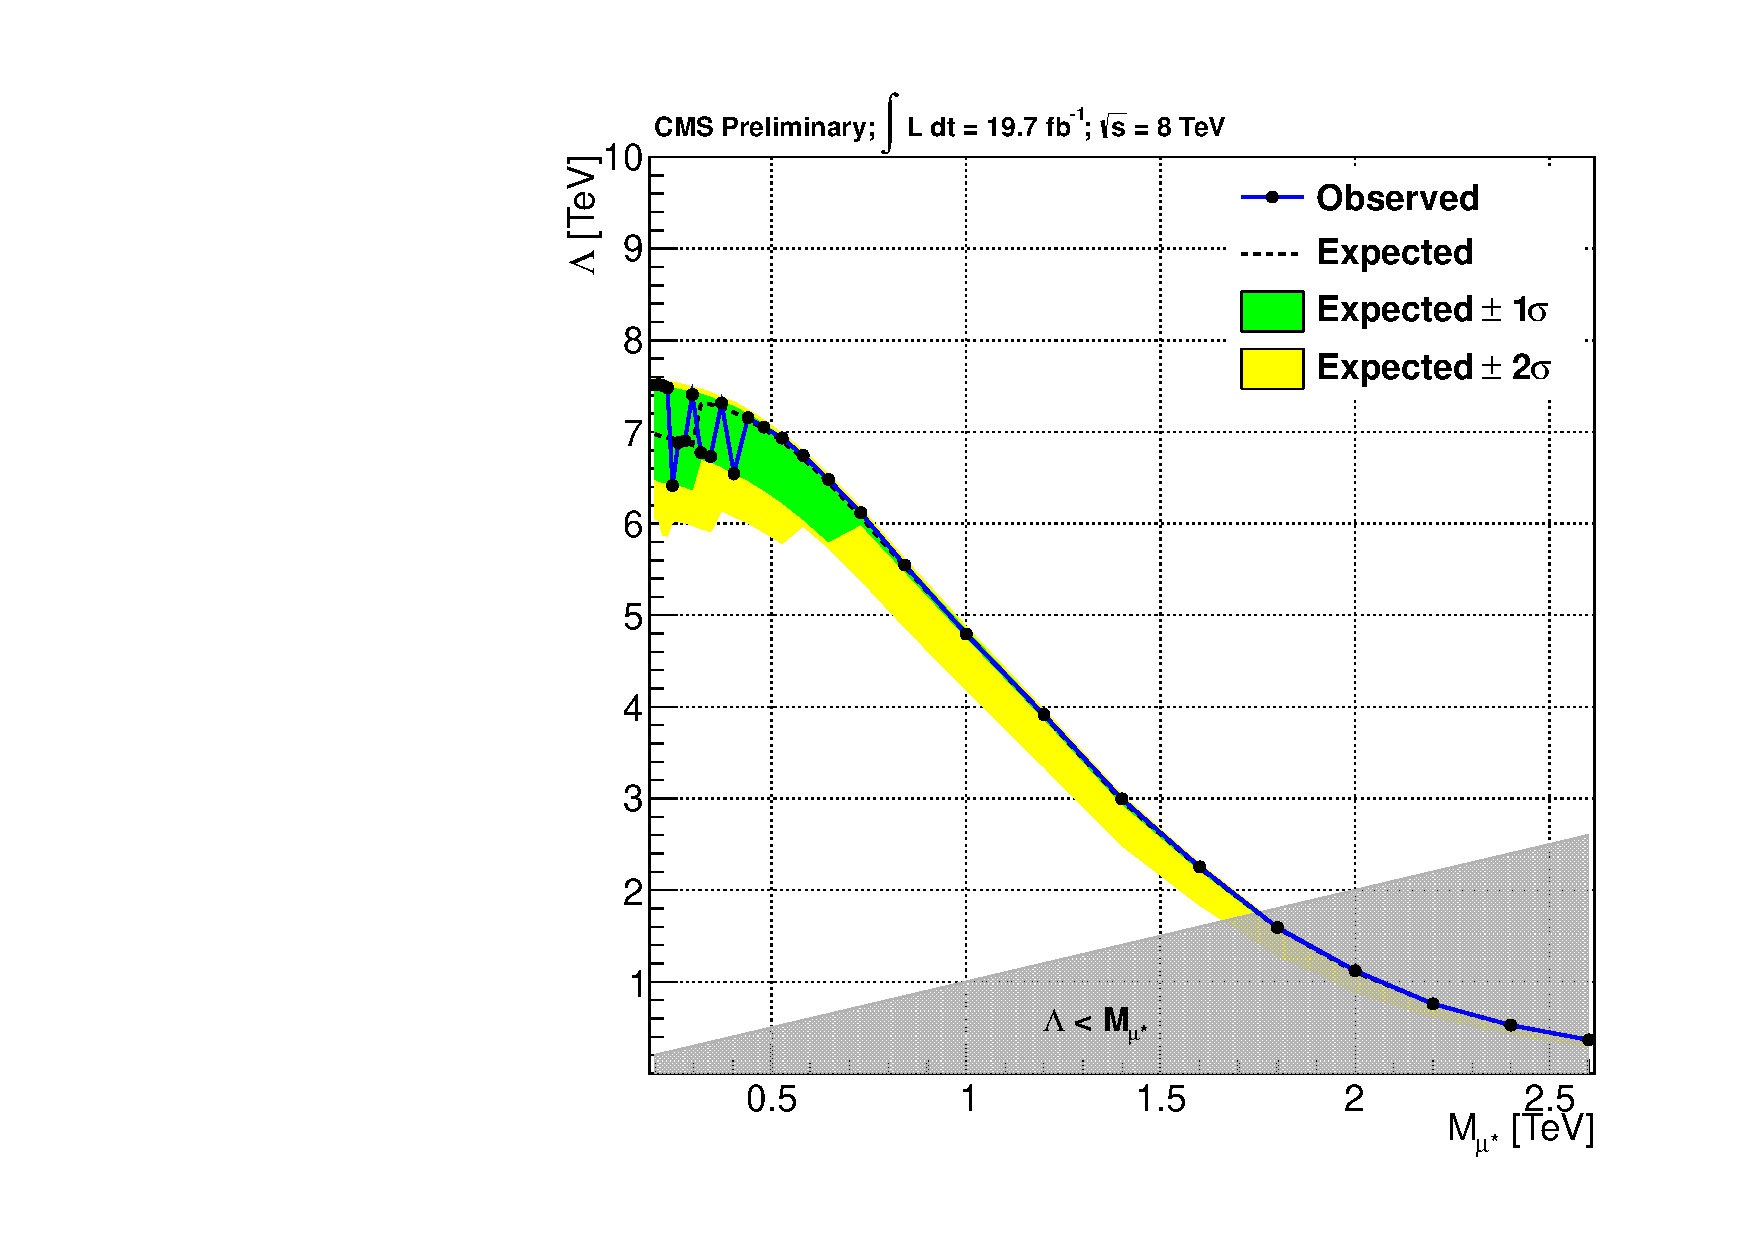
\includegraphics[width=0.48\textwidth]{plot/limit_lambda_combined_mustar.pdf}
\end{center}
\caption{\label{fig:limitmustar}Combined cross section and $\Lambda$ limit for $\mu\mu^{*} \rightarrow 4l$.}
\end{figure}

\begin{figure}[hp!]
\begin{center}
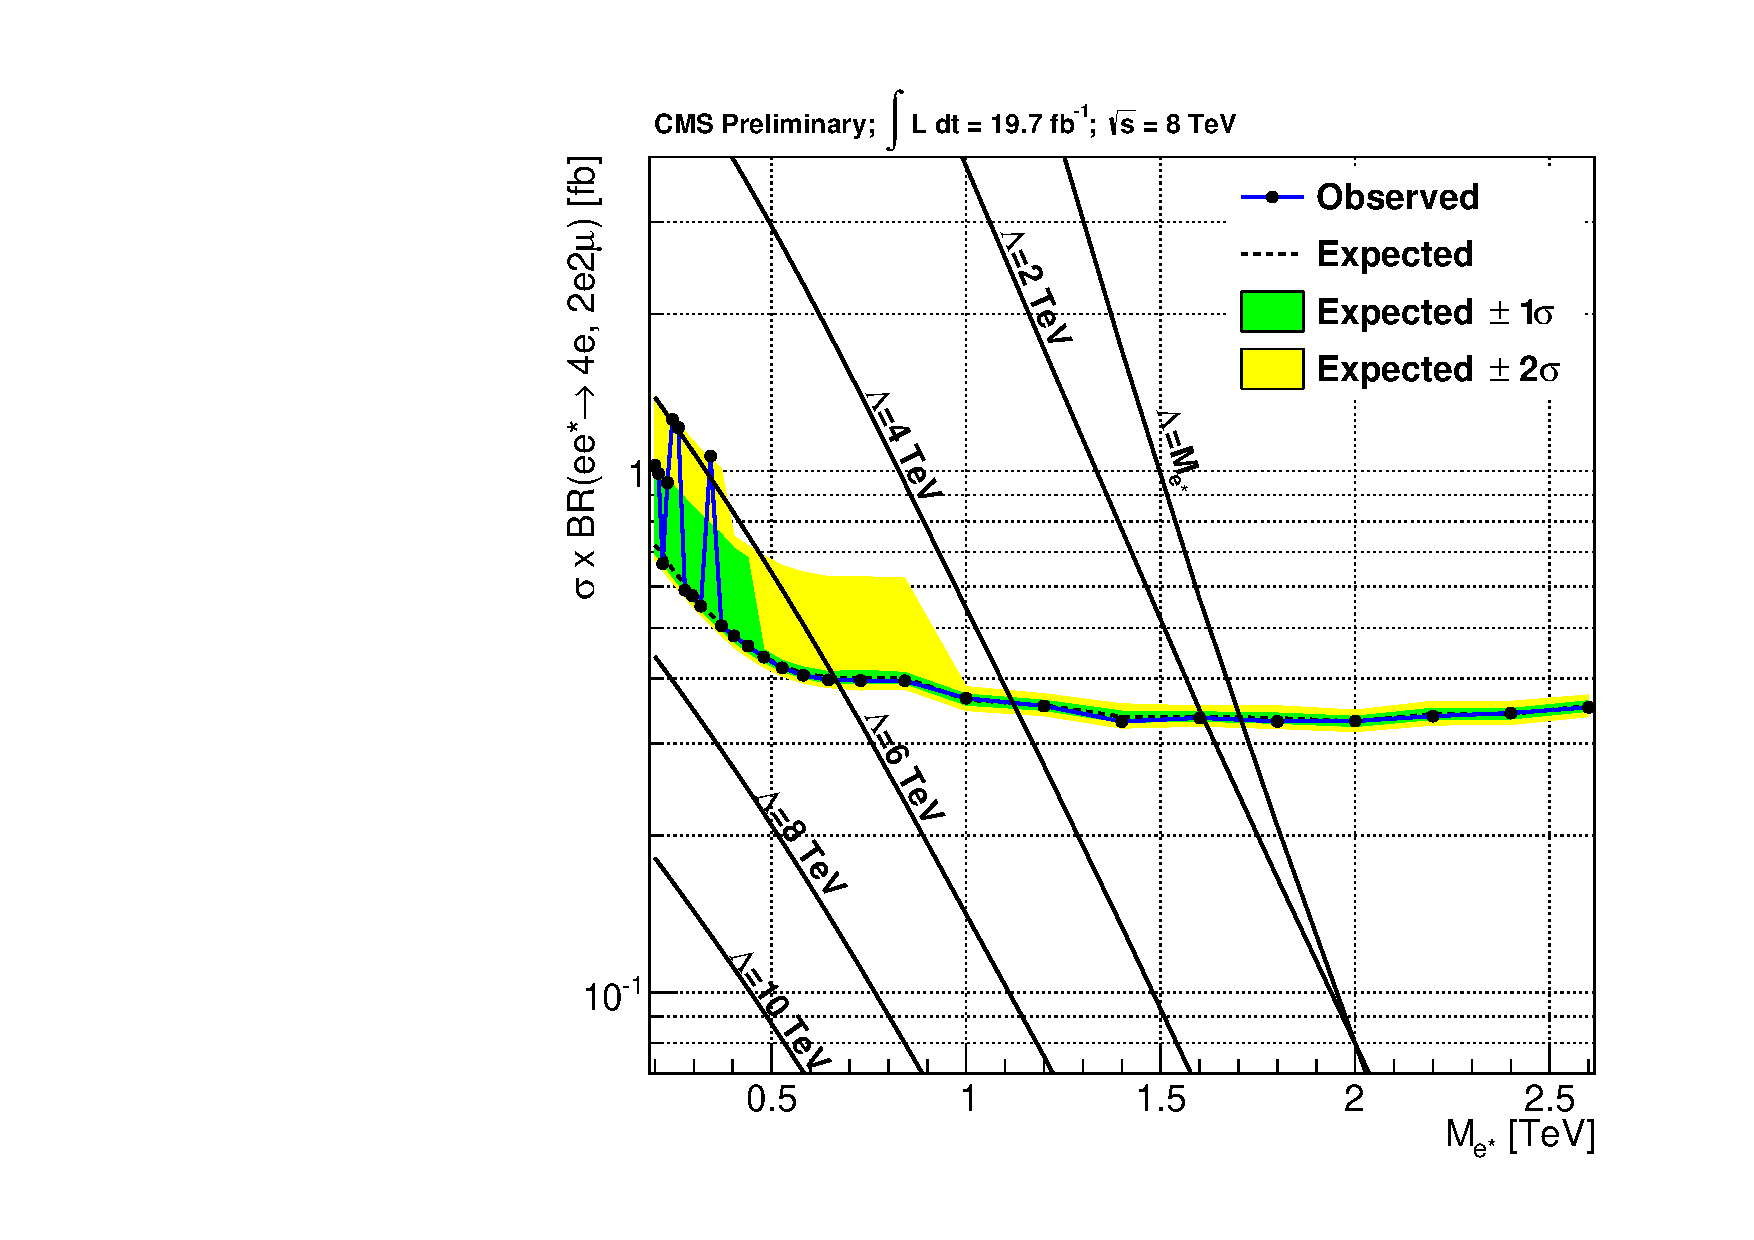
\includegraphics[width=0.48\textwidth]{plot/limit_combined_estar.pdf}
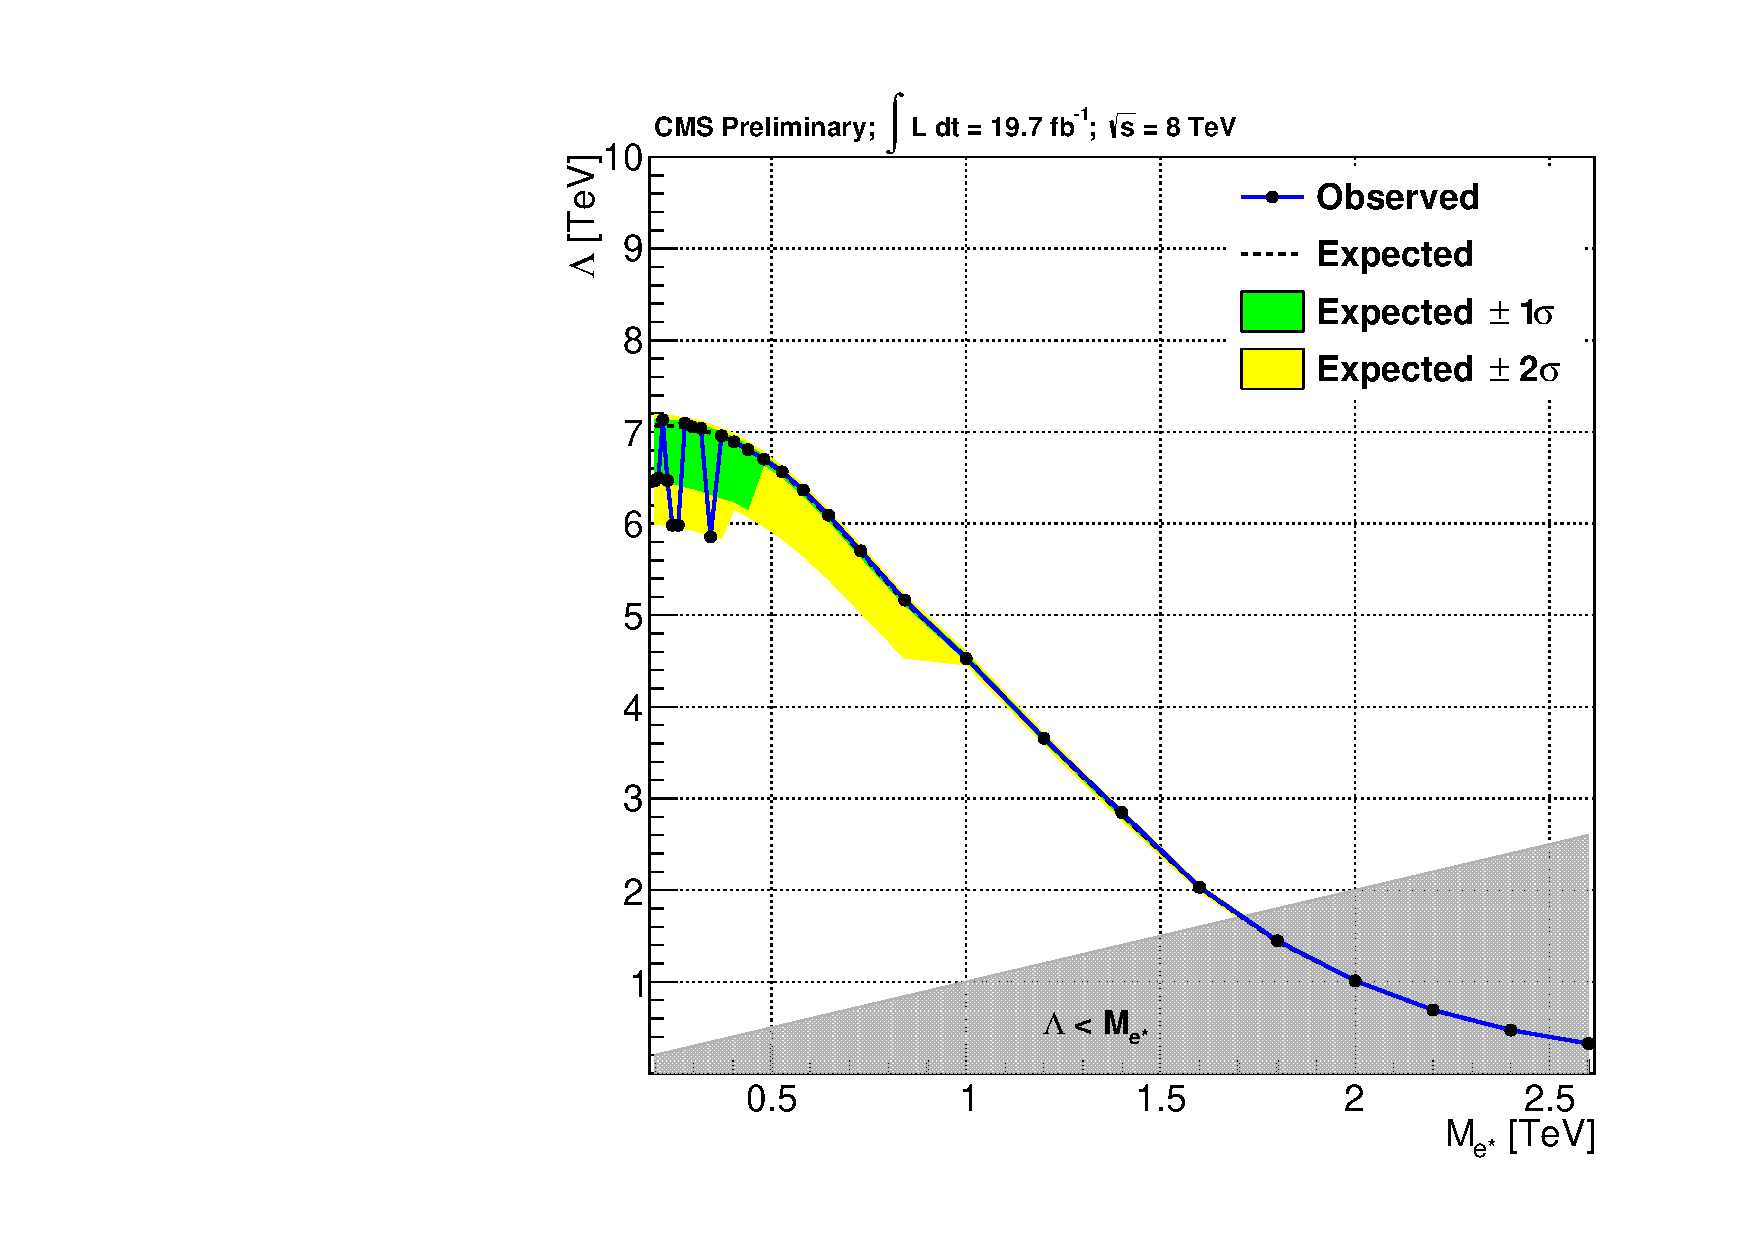
\includegraphics[width=0.48\textwidth]{plot/limit_lambda_combined_estar.pdf}
\end{center}
\caption{\label{fig:limitestar}Combined cross section and $\Lambda$ limit for $e e^{*} \rightarrow 4l$.}
\end{figure}

The limit plots show some striking features. Looking at Fig. \ref{fig:limit4mu} to \ref{fig:limitestar} it can be seen that on the one hand, the error bands are mostly asymmetric around the median expected limit. On the other hand, the $1\sigma$- and sometimes also the $2\sigma$-band drop to a value very close to the dashed line of the median expected limit. Both effects have the same reason which is the low background expectation of below one event in the search regions (comp. Tab. \ref{tab:LShape2} - \ref{tab:LShape4}). During the limit computation, repeatedly toy-experiments are diced. When the background expectation is low, those are manly varied in the upper direction as it is not possible to reach under zero. Thus the asymetric error bands can be explained. When the background expectation becomes even lower as in the high mass search regions, the limit calculation is not able to iterate higher intger event assumptions and one after another, first the $1\sigma$- and later on also the $2\sigma$-quantile drop into the $0$-event assumption resulting in the very narrow error bands.

\section{Conclusion}
For the first time, a search for excited electrons and muons is performed in the channels with four leptons in the final states using pp collision data at $\sqrt{s} = 8 TeV$. No evidence of new physics is observed. Combining the respective two search channels, excited electrons with $M_{e^{∗}} < 1.70 TeV$ and excited muons with $M_{\mu^{∗}} < 1.75 TeV$ are excluded for the compositeness scale equals to the excited lepton mass ($M_{l^{*}} = \Lambda$).


\newpage

